\section{Flavour-tagging performance}\label{sec:impactOfGeometries}

The different geometries described in Section~\ref{sec:Geometries} are compared based on their flavour-tagging performance. The flavour tagging is studied using the LCFIPlus package~\cite{website:LCFIPlus}. \\
The performance of the flavour tagging depends on the jet energy and polar angle. For this reason, the study is done considering dijet events with center-of-mass energies, $\sqrt{s}$, of 91~GeV, 200~GeV, 500~GeV and 1000~GeV having polar angles of $\theta=10^\circ, 20^\circ, ..., 90^\circ$ with a uniform distribution in $\phi$ angles. Initial state radiation (ISR) and beamstrahlung (BS) were switched off during the event generation and hence the final-state quarks are in a back-to-back configuration.\\
For each jet flavour, energy and angle, 80000 events are used for the following processes:
\begin{itemize}
\item e$^+$e$^-$ $\rightarrow$ b\={b}
\item e$^+$e$^-$ $\rightarrow$ c\={c}
\item e$^+$e$^-$ $\rightarrow$ u\={u}
\item e$^+$e$^-$ $\rightarrow$ d\={d}
\item e$^+$e$^-$ $\rightarrow$ s\={s}
\end{itemize}

The boosted decision trees (BDTs) are trained using 50\% of the generated events and the other 50\% are used for testing the performance of the flavour tagging.
%% The software versions used are given in Table \ref{tab:softwareVersions}:

%% \begin{table}[H]
%%   \caption{Software versions used for the flavour tagging.}
%%   \begin{center}
%%     \begin{tabular}{ c c}
%%       \hline
%%       Software & Version \\ \hline \hline
%%       SLIC & v3r0p3 \\ \hline
%%       org.lcsim & 2.5 \\ \hline
%%       LCFIPlus & v0.52 \\ \hline
%%     \end{tabular}
%%   \end{center}
%%   \label{tab:softwareVersions}
%% \end{table}

\subsection{Jet-energy dependence}
The dependence of the flavour-tagging performance on the jet energy is shown in Figures \ref{fig:FTEnergyDependenceB} and \ref{fig:FTEnergyDependenceC} using the \begin{it}spirals\end{it} geometry and dijet events at different center-of-mass energies with a mixture of all considered polar angles. \\
In Figure~\ref{fig:FTEnergyDependenceB}, the fake rate of recognising charm and light flavour (LF) jets as beauty jets is plotted versus the b-tag efficiency. In Figure~\ref{fig:FTEnergyDependenceC}, the fake rate of recognising beauty and light flavour jets as charm jets is plotted versus the c-tag efficiency. \\
In general, the b-tag performance is better for jets with lower
energies. This can be explained by the fact that a B hadron with lower
energy has a shorter decay length and therefore decays most likely
before the first barrel layer of the vertex detector, while a B hadron with higher energy
decays sometimes after the first layer. This leads to a degradation of
the track reconstruction and thus the vertex finding and flavour
tagging for high-energy jets.

\begin{figure}[H]
        \begin{subfigure}[b]{0.5\textwidth}
          \centering
          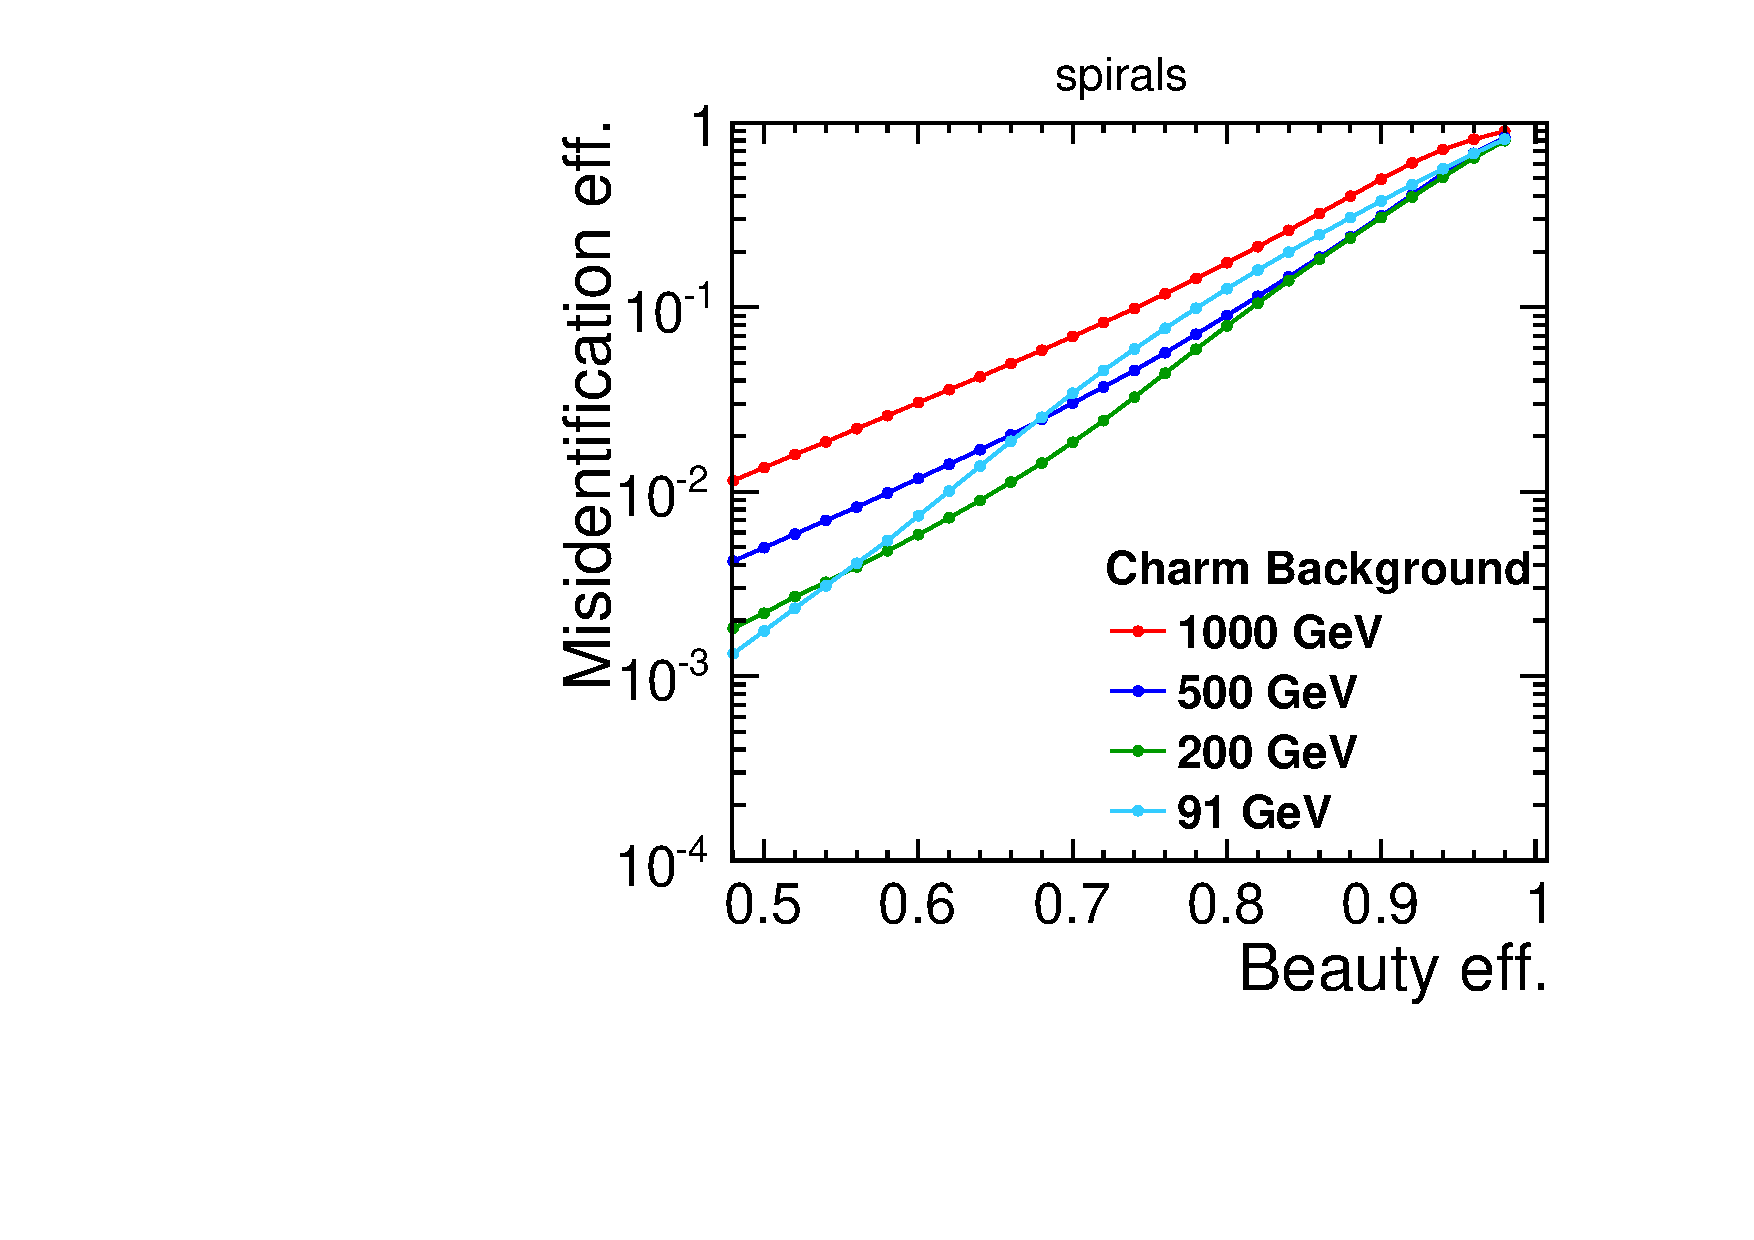
\includegraphics[width=\textwidth]{Figures/ImpactOfGeometries/Global_energies_CLIC_SiD_spirals_Beauty_Charm_.pdf}
          \caption{}
          \label{}
        \end{subfigure}%
        ~ 
        \begin{subfigure}[b]{0.5\textwidth}
          \centering
          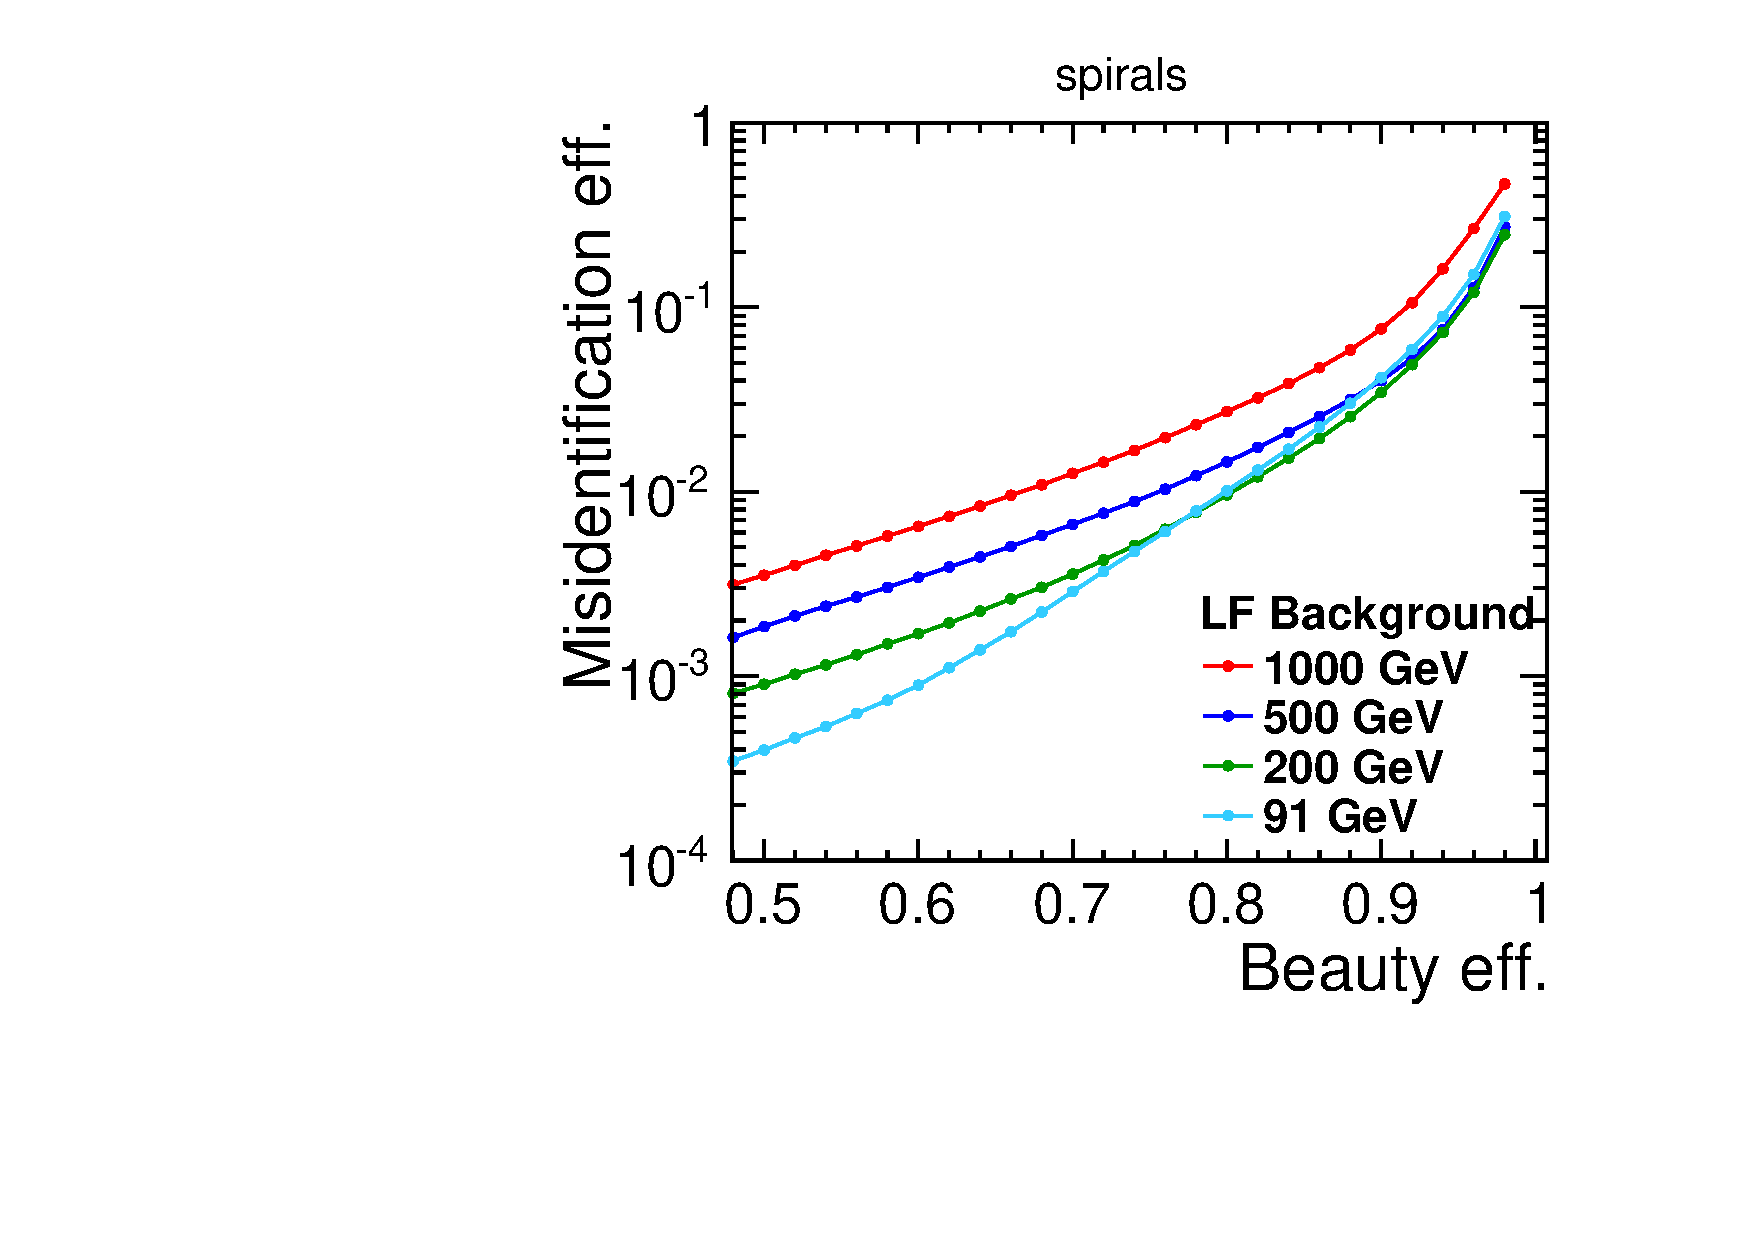
\includegraphics[width=\textwidth]{Figures/ImpactOfGeometries/Global_energies_CLIC_SiD_spirals_Beauty_LF_.pdf}
          \caption{}
          \label{}
        \end{subfigure}
        \caption{b-tag efficiencies and fake rates for dijets at a
          mixture of polar angles between $10^{\circ}$ and
          $90^{\circ}$ for the \textit{spirals} geometry. (a) shows the fake rate for recognising charm jets as beauty jets and (b) shows the fake rate for recognising light flavour jets as beauty jets.}\label{fig:FTEnergyDependenceB}
\end{figure}

\begin{figure}[H]
        \begin{subfigure}[b]{0.5\textwidth}
          \centering
          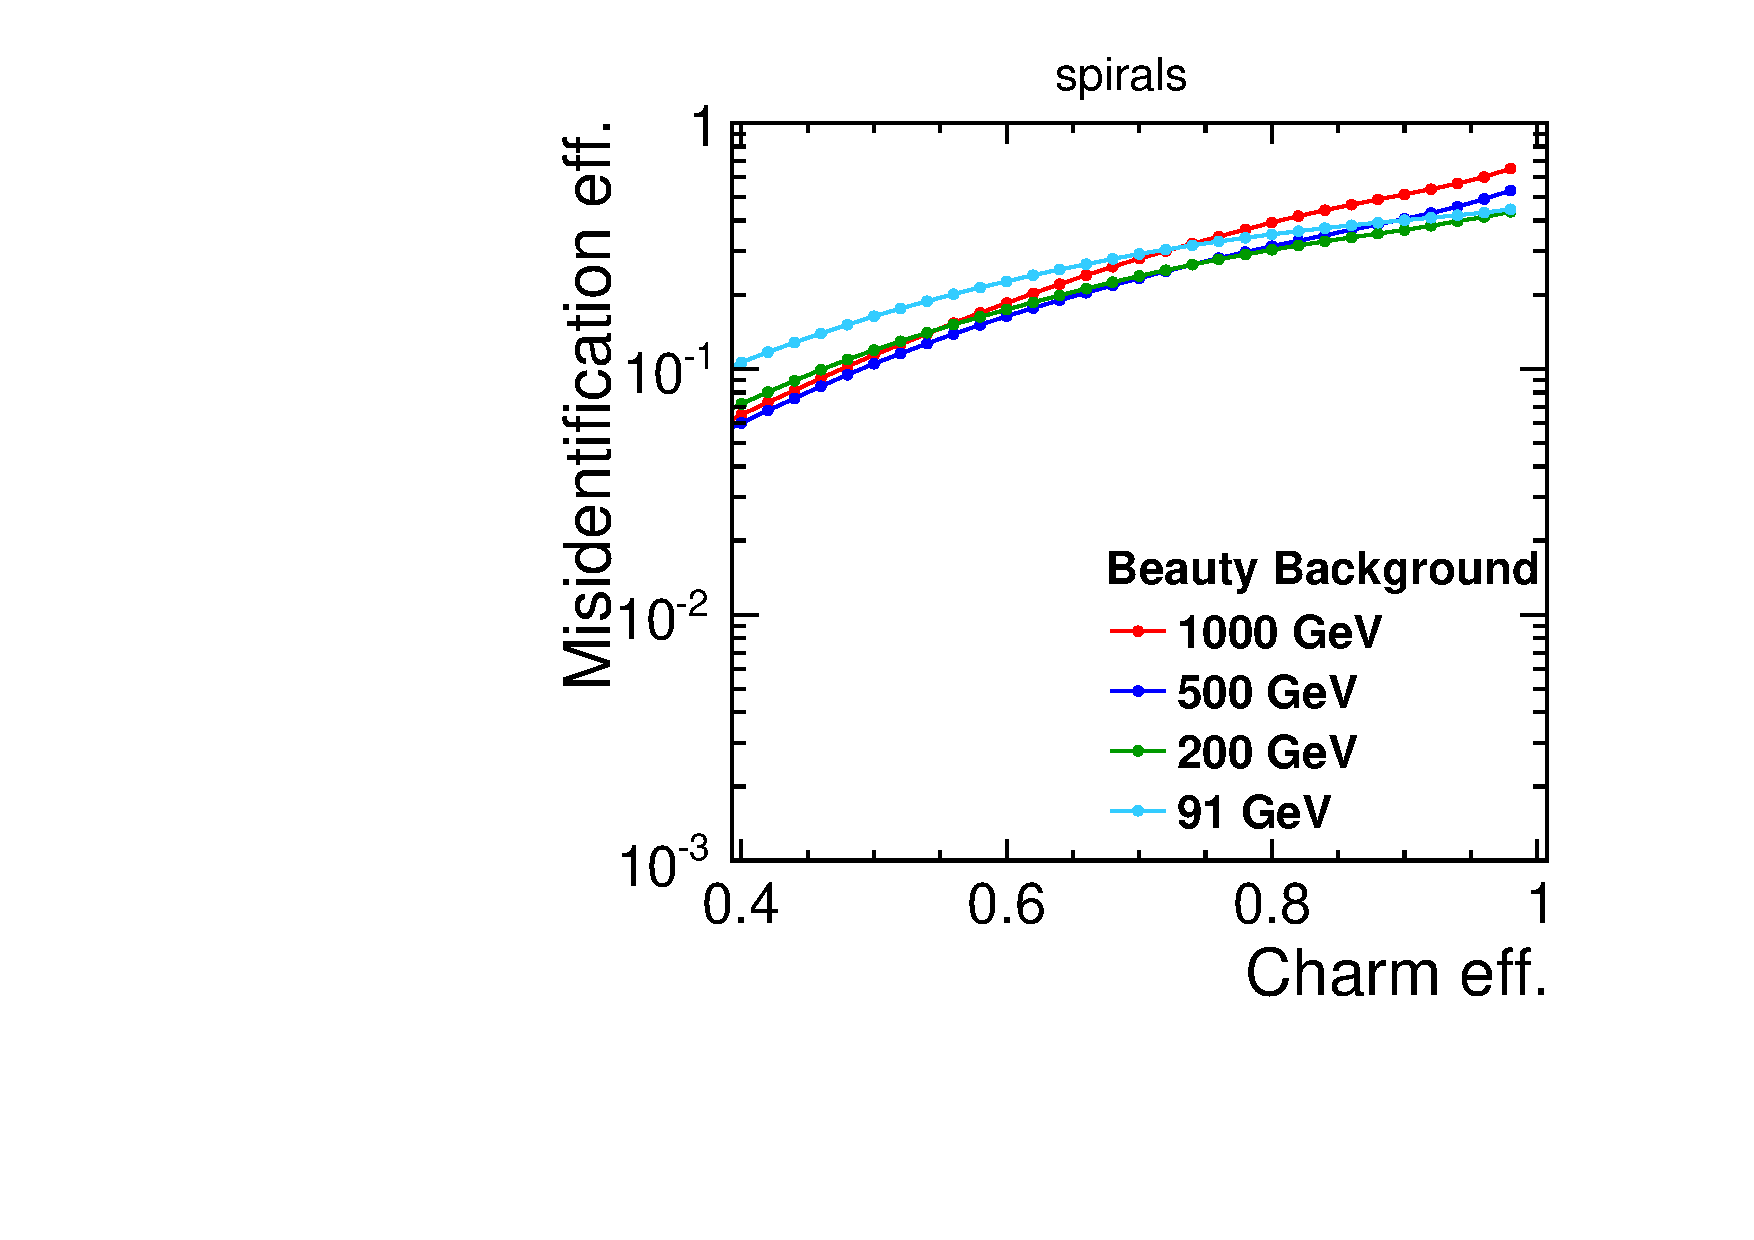
\includegraphics[width=\textwidth]{Figures/ImpactOfGeometries/Global_energies_CLIC_SiD_spirals_Charm_Beauty_.pdf}
          \caption{}
          \label{}
        \end{subfigure}%
        ~ 
        \begin{subfigure}[b]{0.5\textwidth}
          \centering
          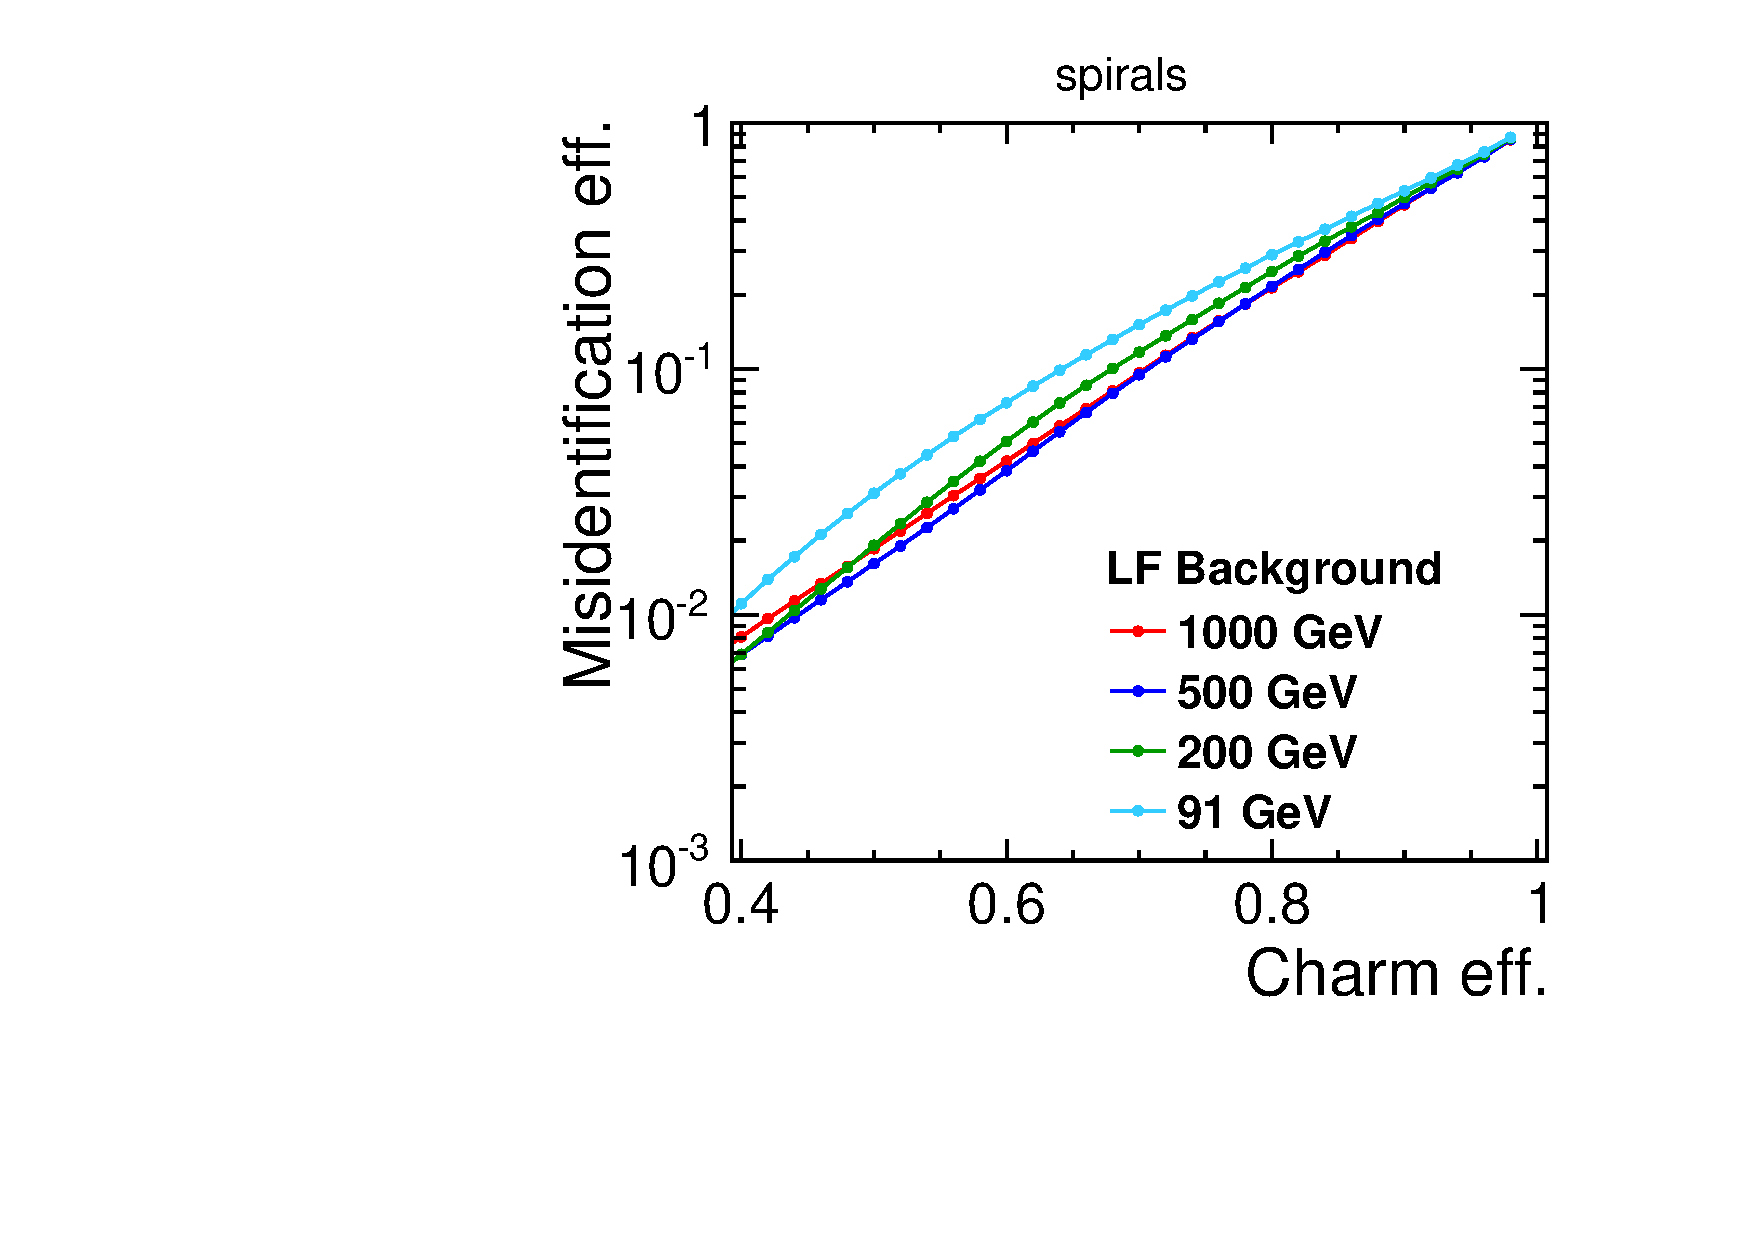
\includegraphics[width=\textwidth]{Figures/ImpactOfGeometries/Global_energies_CLIC_SiD_spirals_Charm_LF_.pdf}
          \caption{}
          \label{}
        \end{subfigure}
        \caption{c-tag efficiencies and fake rates for dijets at a mixture of angles between $10^{\circ}$ and
          $90^{\circ}$ for the \textit{spirals} geometry. (a) shows the fake rate for recognising beauty jets as charm jets and (b) shows the fake rate for recognising light flavour jets as charm jets.}\label{fig:FTEnergyDependenceC}
\end{figure}

\subsection{Jet-angle dependence}
The dependence of the flavour-tagging performance on the jet polar angle is shown in Figures \ref{fig:FTAngleDependenceB} and \ref{fig:FTAngleDependenceC} using the \begin{it}spirals\end{it} geometry for jets in dijet events at $\sqrt{s}=$200~GeV. \\
In the forward region, several factors are causing the sizeable decrease in performance. For low polar angles, some fraction of particles in the jets is not reconstructed along the beam axis. In addition, the vertex detector resolution in
the forward region is worse than in the other parts due to the large
distance between the reconstructed vertex and the sensors (cf. Figures
\ref{fig:spiralRes} and \ref{fig:doubleLayerRes}). In addition, the number of
sensitive layers decreases with decreasing polar angles (cf. Figure~\ref{fig:vertex_nb_layer}). \\
%% In these Figures the errors on the efficiencies are shown to give an
%% idea of the magnitude of the uncertainties. When we compute an efficiency, we select some events among all available events and the uncertainty on the selection is given by Binomial errors. The error is given by: $\sqrt{{e \cdot (1 -e)} \over m}$, where $e$ is the efficiency and $m$ the total number of jets. The errors on the computed efficiencies are very small (around $10^{-4}$). \\
To illustrate the size of the fluctuations due to the finite size of the event samples used, the statistical uncertainties of the obtained misidentification efficiencies are shown by error bars which are negligible.
More results for different jet energies and detector geometries can be found in Appendices~\ref{sec:CDR_jet_angle}, \ref{sec:spirals_jet_angle} and \ref{sec:doubleSpirals_jet_angle}.
\begin{figure}[H]
  \begin{subfigure}[b]{0.5\textwidth}
    \centering
    \begin{tikzpicture}
      \node[anchor=south west,inner sep=0] (image) at (0,0){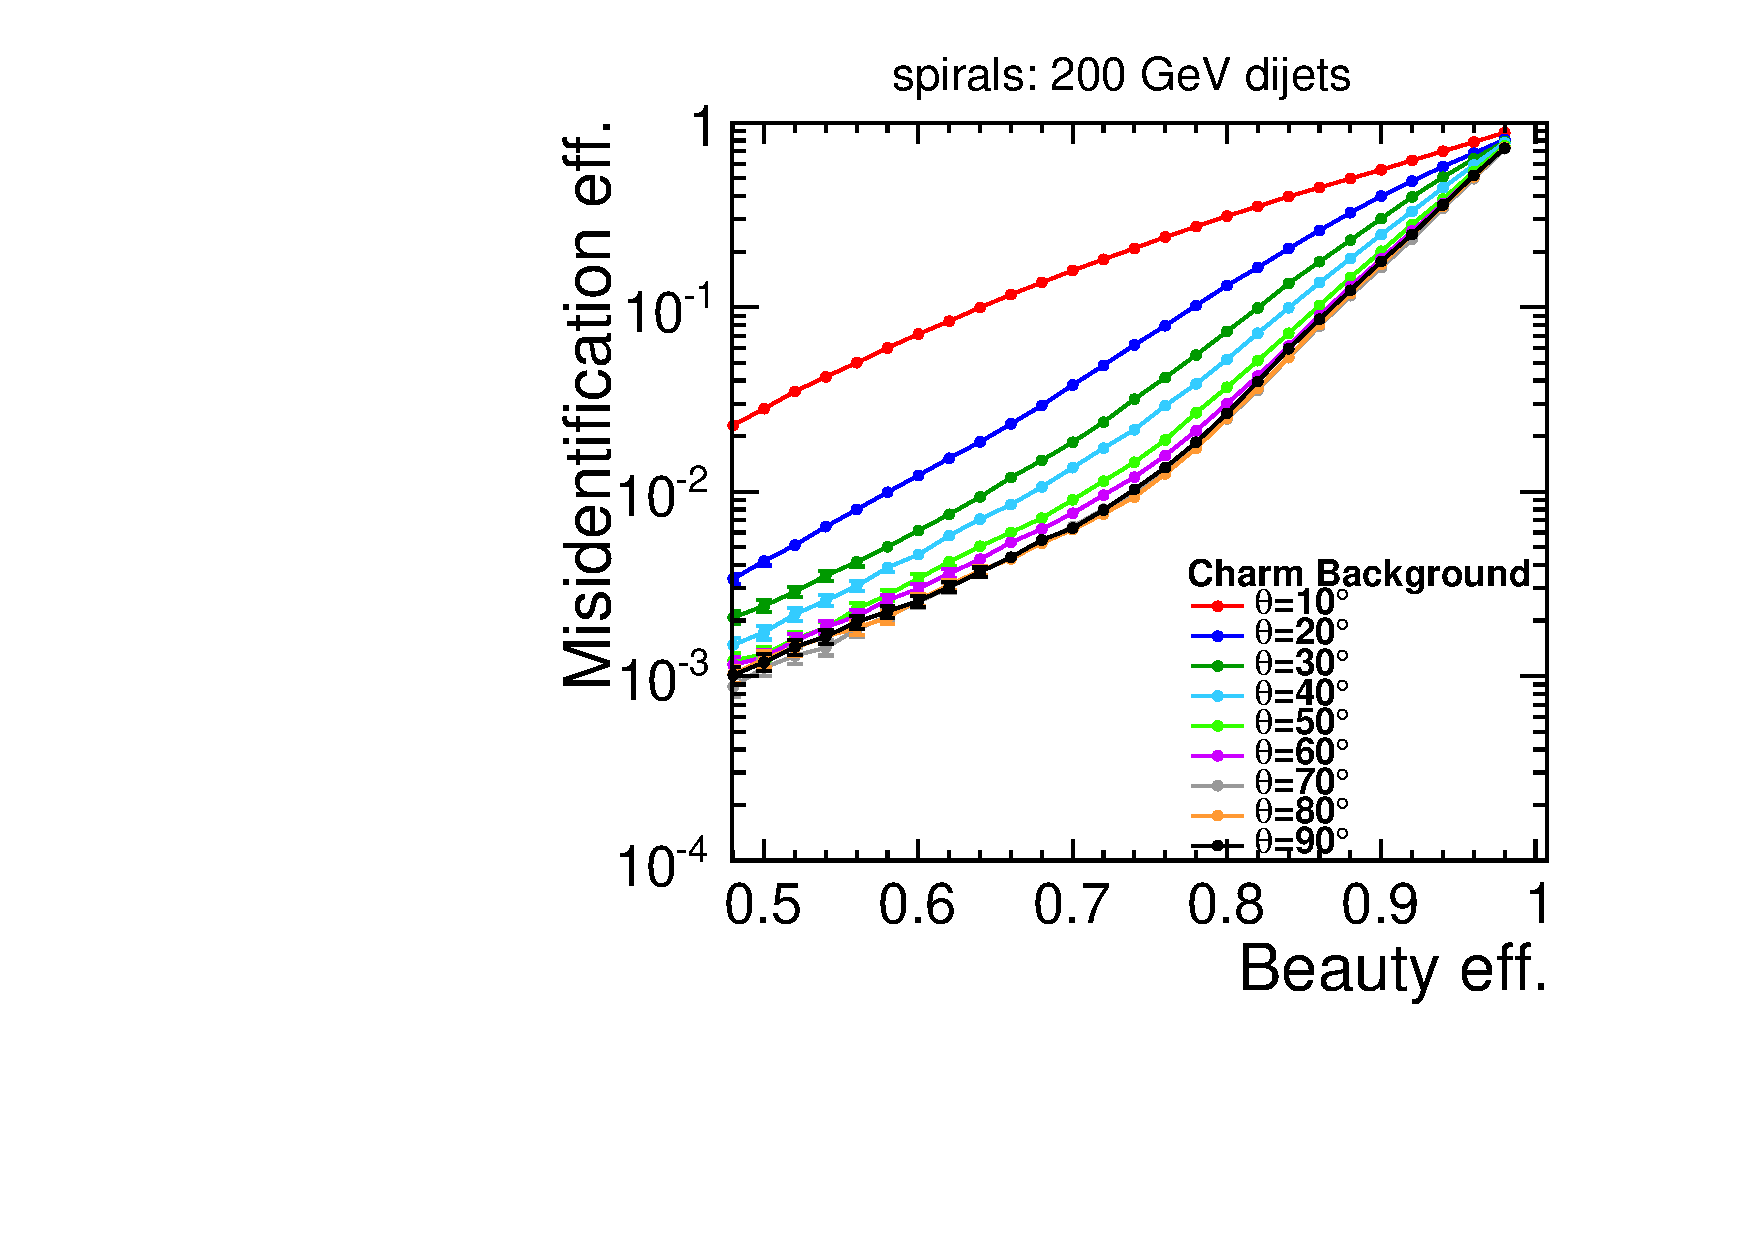
\includegraphics[width=\textwidth]{Figures/ImpactOfGeometries/allAngles_CLIC_SiD_spirals_Beauty_Charm_200.pdf}};
      \draw[white, fill=white] (1.8, 6.3) rectangle (5.7, 7);
    \end{tikzpicture}
    \caption{}
    \label{}
  \end{subfigure}%
  ~ 
  \begin{subfigure}[b]{0.5\textwidth}
    \centering
    \begin{tikzpicture}
      \node[anchor=south west,inner sep=0] (image) at (0,0){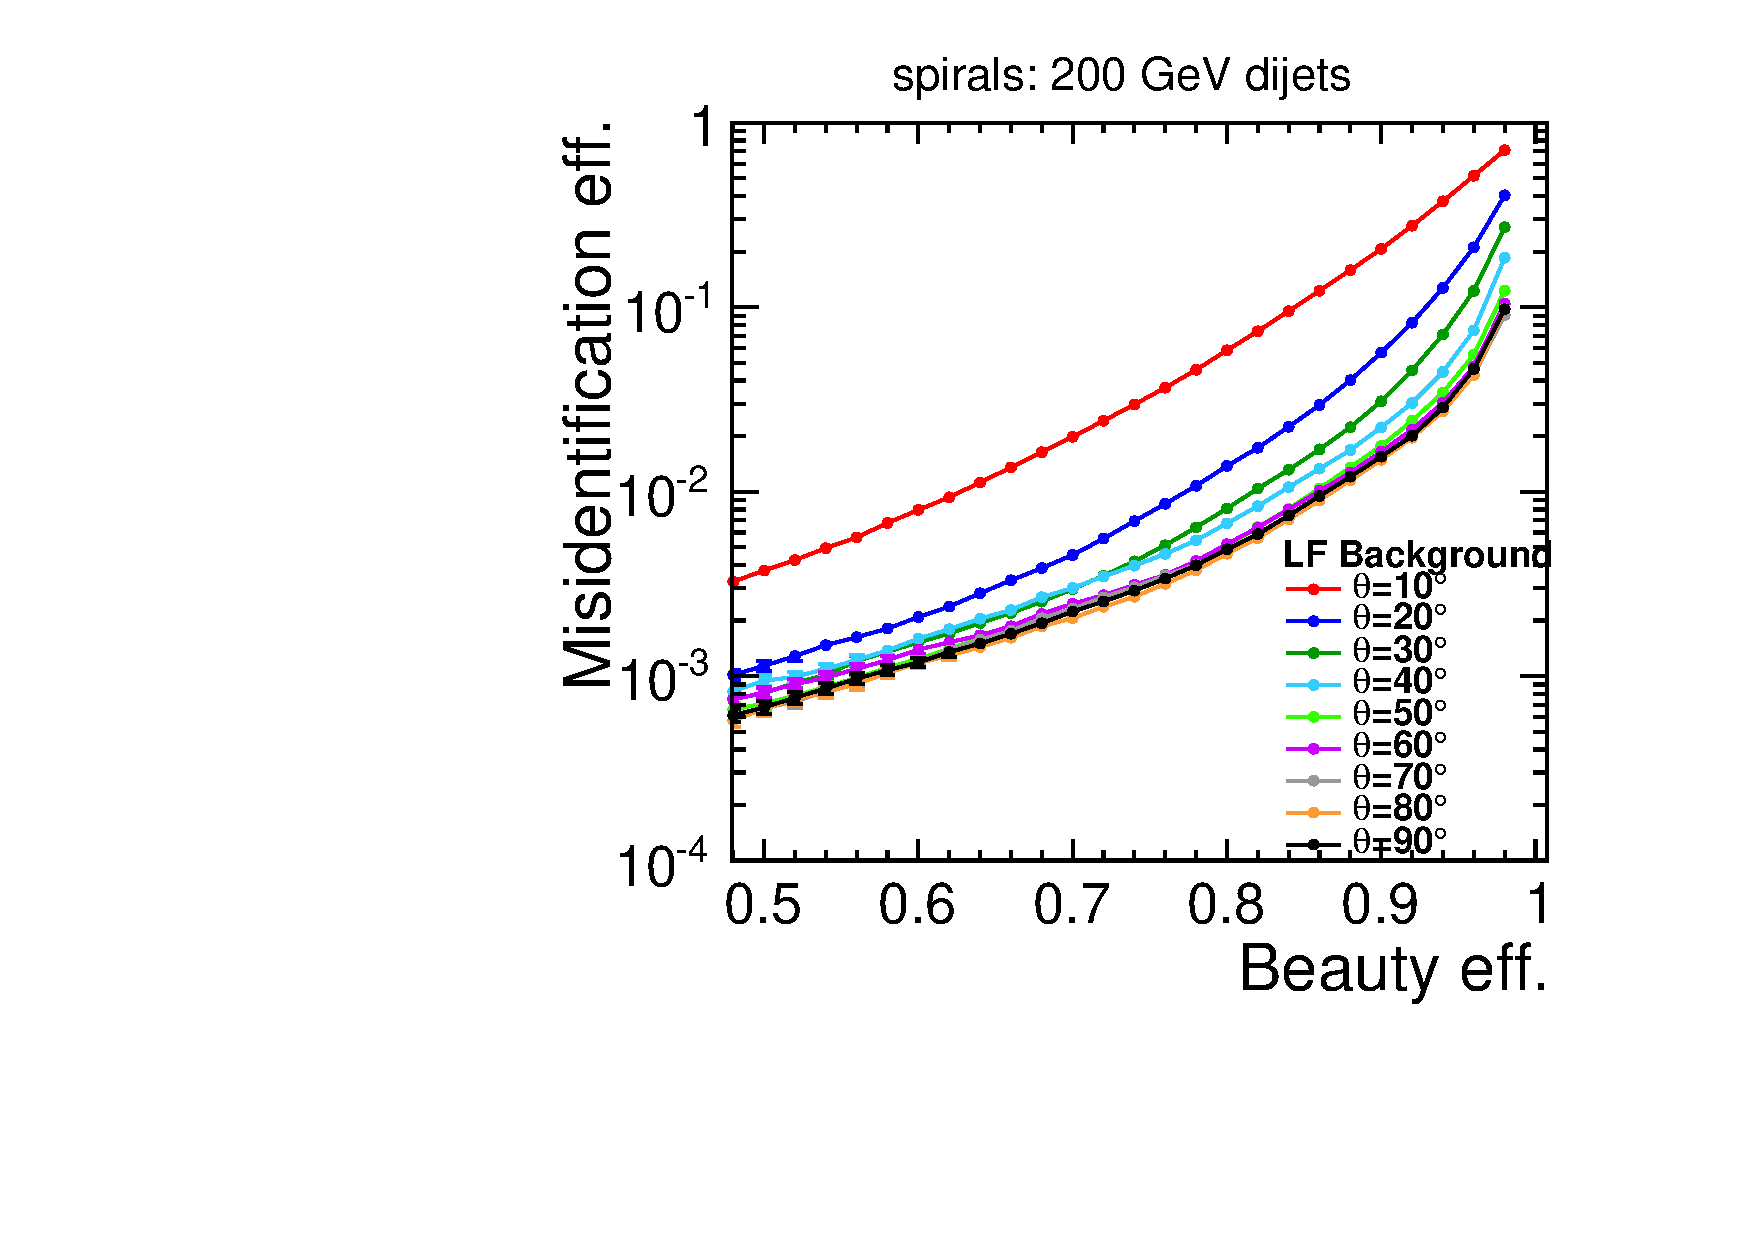
\includegraphics[width=\textwidth]{Figures/ImpactOfGeometries/allAngles_CLIC_SiD_spirals_Beauty_LF_200.pdf}};
      \draw[white, fill=white] (1.8, 6.3) rectangle (5.7, 7);
    \end{tikzpicture}
    \caption{}
    \label{}
  \end{subfigure}
  \caption{b-tag efficiencies for jets in dijet events at $\sqrt{s}=200$~GeV with different polar angles using the \textit{spirals} geometry. (a) shows the fake rate for recognising charm jets as beauty jets and (b) shows the fake rate for recognising light flavour jets as beauty jets.}\label{fig:FTAngleDependenceB}
\end{figure}

\begin{figure}[H]
  \begin{subfigure}[b]{0.5\textwidth}
    \centering
    \begin{tikzpicture}
      \node[anchor=south west,inner sep=0] (image) at (0,0){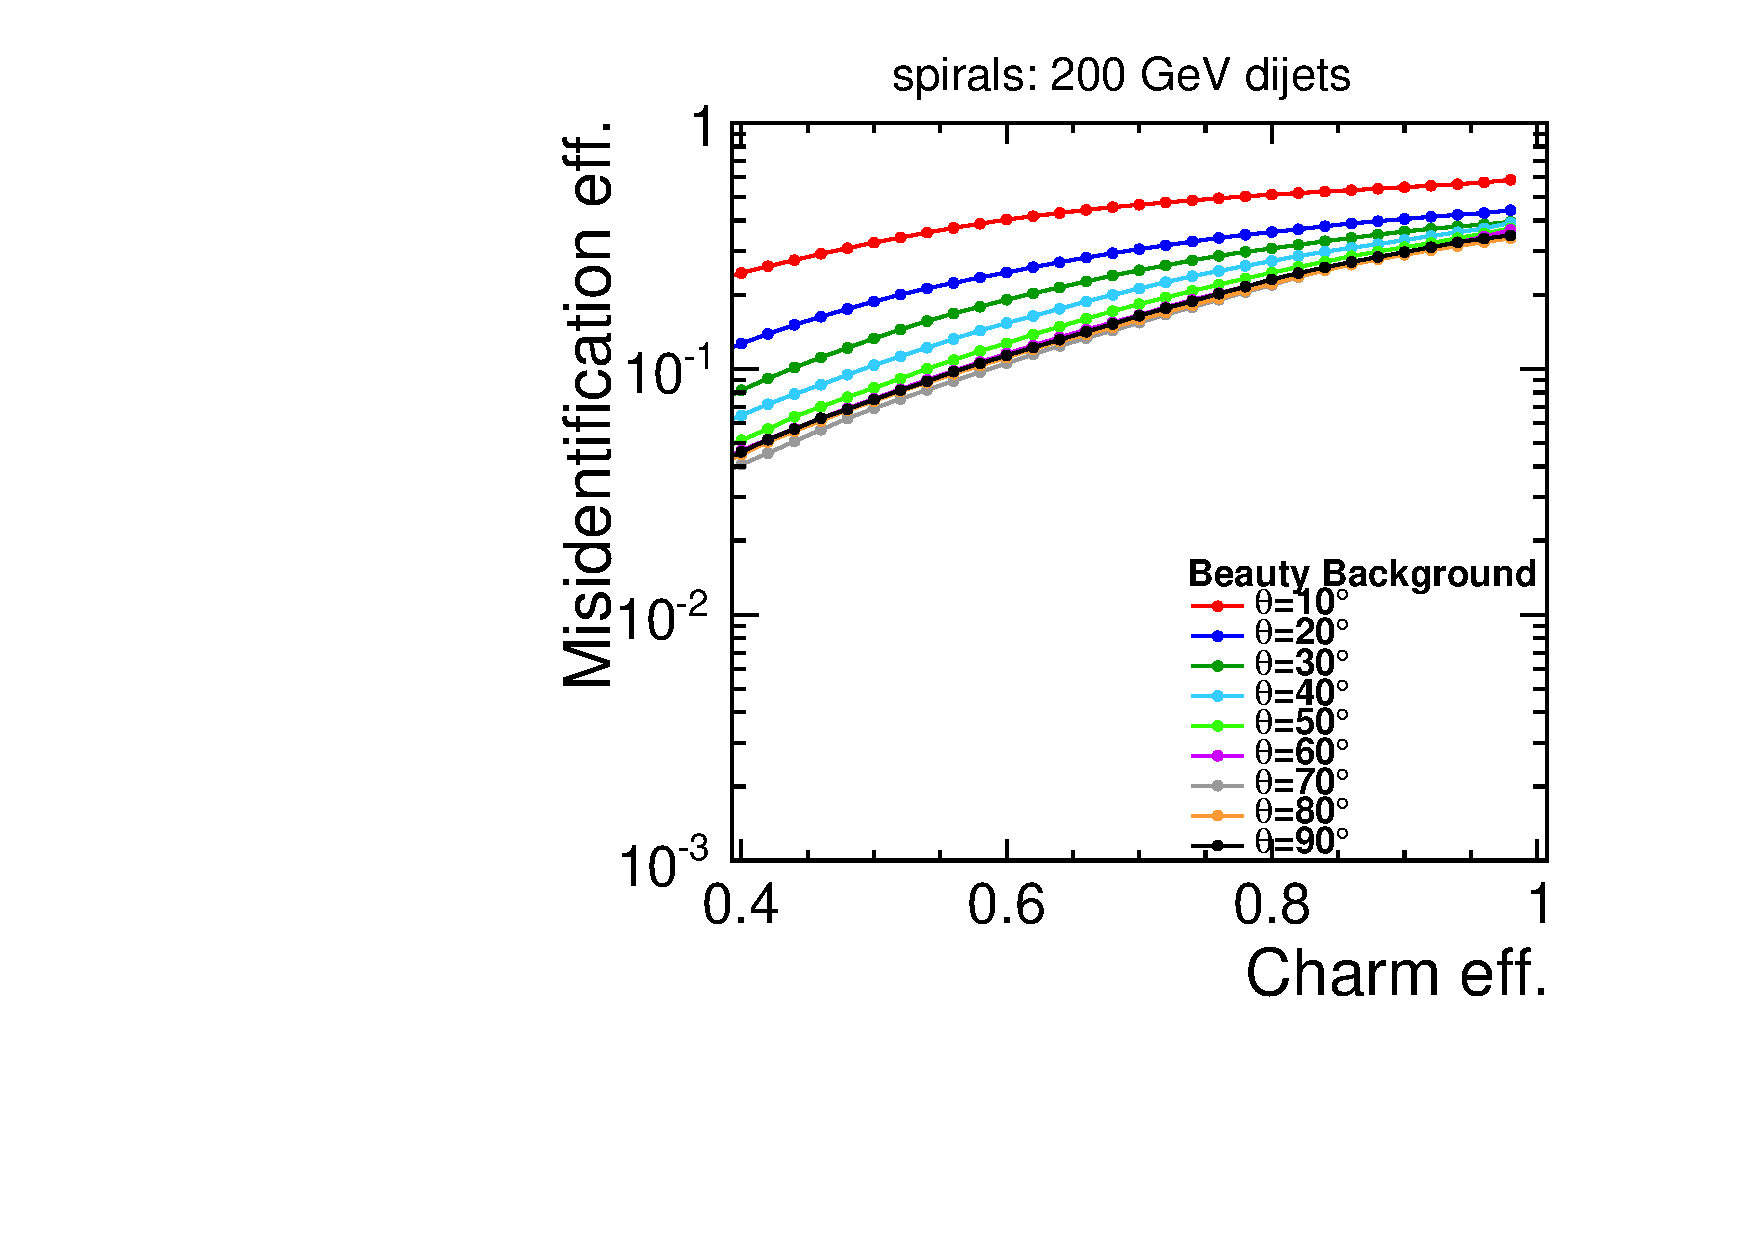
\includegraphics[width=\textwidth]{Figures/ImpactOfGeometries/allAngles_CLIC_SiD_spirals_Charm_Beauty_200.pdf}};
      \draw[white, fill=white] (1.8, 6.3) rectangle (5.7, 7);
    \end{tikzpicture}
    \caption{}
    \label{}
  \end{subfigure}%
  ~ 
  \begin{subfigure}[b]{0.5\textwidth}
    \centering
    \begin{tikzpicture}
      \node[anchor=south west,inner sep=0] (image) at (0,0){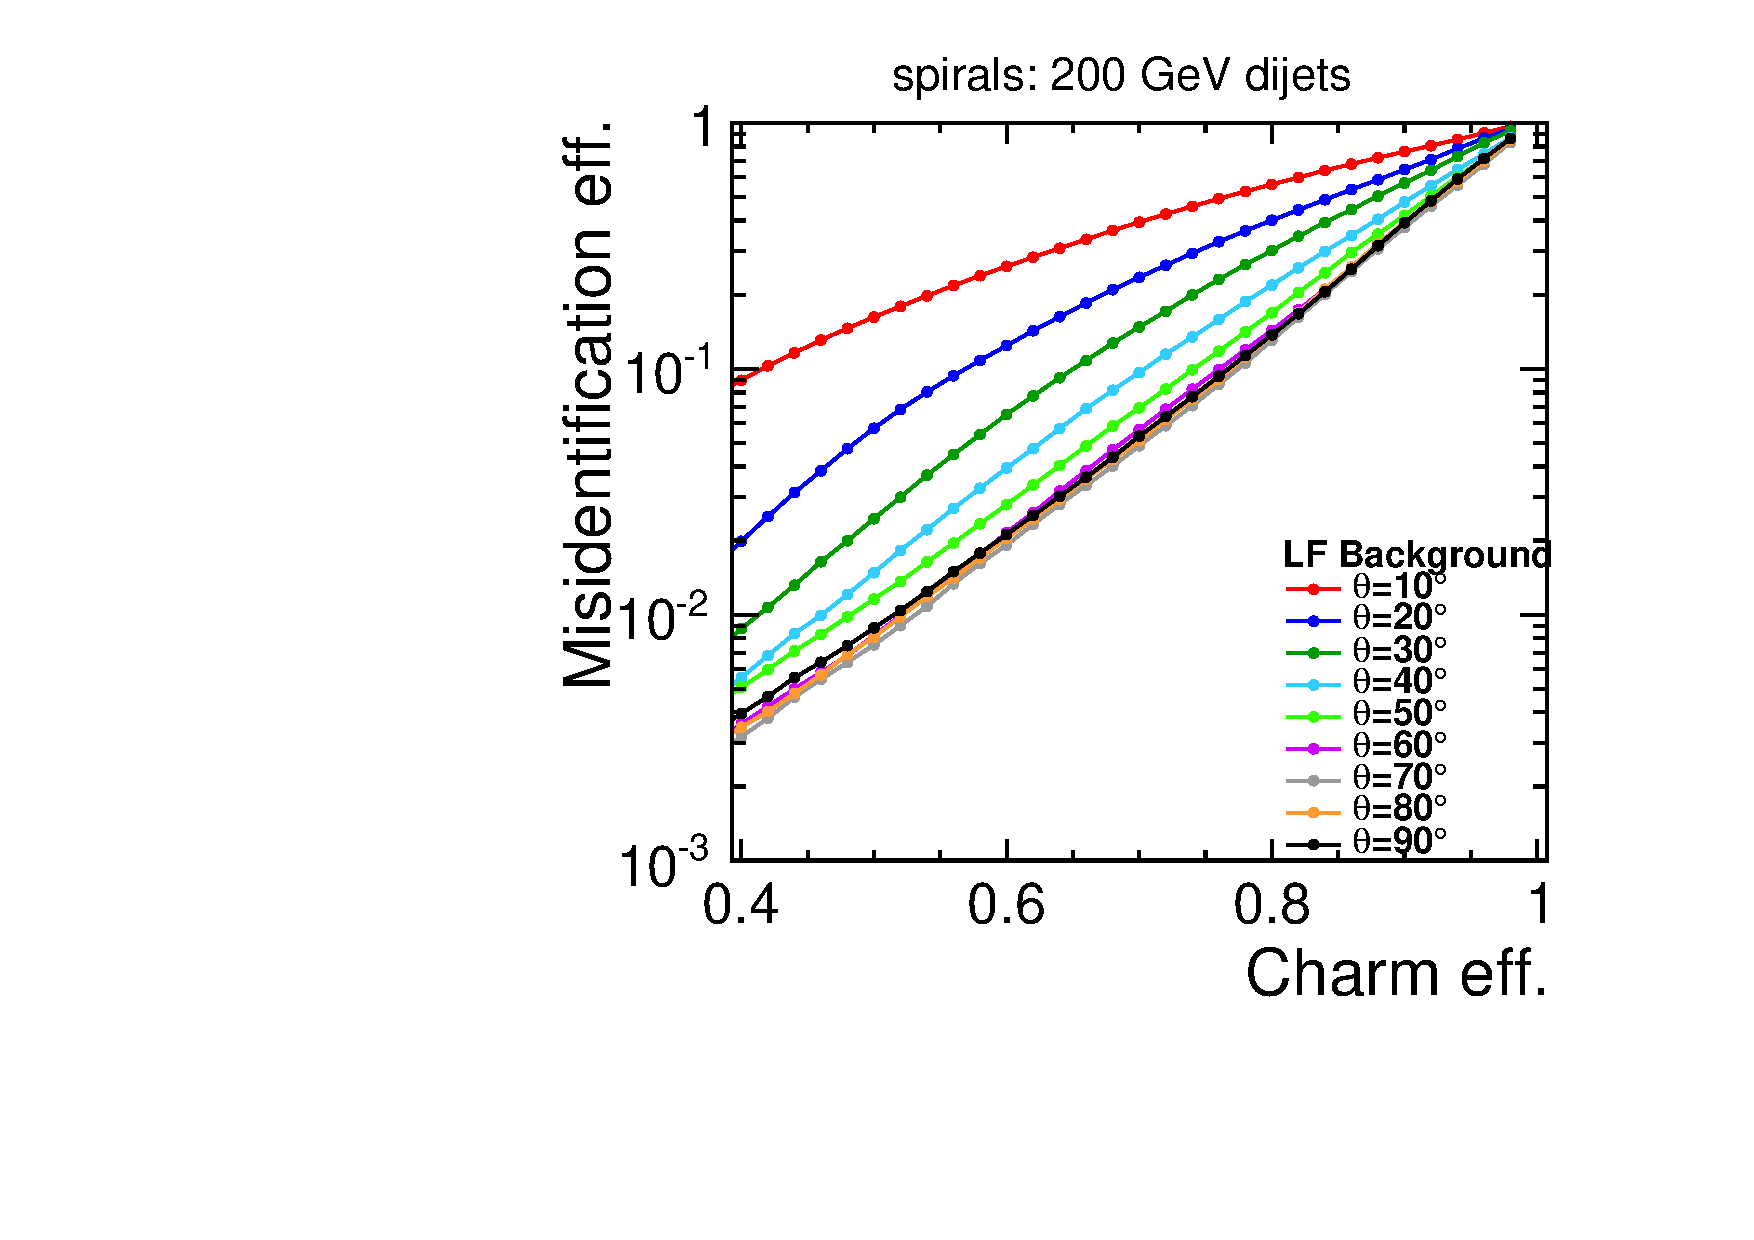
\includegraphics[width=\textwidth]{Figures/ImpactOfGeometries/allAngles_CLIC_SiD_spirals_Charm_LF_200.pdf}};
      \draw[white, fill=white] (1.8, 6.3) rectangle (5.7, 7);
    \end{tikzpicture}
    \caption{}
    \label{}
  \end{subfigure}
  \caption{c-tag efficiencies for jets in dijet events at $\sqrt{s}=200$~GeV with different polar angles using the \textit{spirals} geometry. (a) shows the fake rate for recognising beauty jets as charm jets and (b) shows the fake rate for recognising light flavour jets as charm jets.}\label{fig:FTAngleDependenceC}
\end{figure}

\subsection{Comparison of different layouts}

In the following sections, the different geometries are compared based on their flavour-tagging performance. First, the spiral configuration is compared to the disks in the endcap regions. Then, the double-layered sensors are compared to the single-layered sensors. Finally, the \textit{double\_spirals} geometry is compared to the CDR geometry.


%% \begin{figure}[H]
%%   \centering
%%   \includegraphics[scale=0.4]{Figures/}
%%   \caption{}
%%   \label{}
%% \end{figure}

%----------------------------------------------------------------------
\subsubsection{\emph{spirals} and CDR}\label{sec:spirals_CDR}

In order to compare two geometries in terms of flavour-tagging performance, the ratio between the misidentification probabilities is computed. \\
Figures \ref{fig:spirals_disks_beauty} and \ref{fig:spirals_disks_charm} compare the CDR and the \textit{spirals} geometry using jets in dijet events at $\sqrt{s}=200$~GeV with polar angles of $\theta=10^\circ, 20^\circ, 30^\circ$ and $40^\circ$. If the ratio between the misidentification probabilities is smaller than one, then the \textit{spirals} geometry has a better flavour-tagging performance than the CDR geometry. Otherwise, the CDR geometry has a better performance.
In general, the two geometries have a similar performance. However, the b-tagging performance is up to $20\%$ worse using the \textit{spirals} geometry for jets at $\theta=40^{\circ}$. At this angle, there is the transition between the vertex endcaps and the barrel region. With the spiral configuration, the number of sensitive layers becomes dependent on the azimuthal angle $\phi$. Less layers can be hit for the spiral configurations in certain ranges in the azimuthal angle $\phi$ compared to the CDR geometry where the number of layers in the endcap regions does not depend on $\phi$ (cf. Figure~\ref{fig:nbLayers_theta_phi}). The track-finding algorithm requires a minimum number of layers hit in the vertex detector. This requirement is not dependent on the $\phi$ direction of the track. Hence with the current software implementation, it is more likely that tracks in a certain $\phi$ region are missed compared to the CDR geometry. This can be improved in future tracking code with using a $\phi$-dependent optimisation of the track finding strategy. \\
More results for different jet energies can be found in Appendix~\ref{sec:appendix_spirals_vs_CDR}.

\begin{figure}[H]
  \begin{subfigure}[b]{0.5\textwidth}
    \centering
    \begin{tikzpicture}
      \node[anchor=south west,inner sep=0] (image) at (0,0){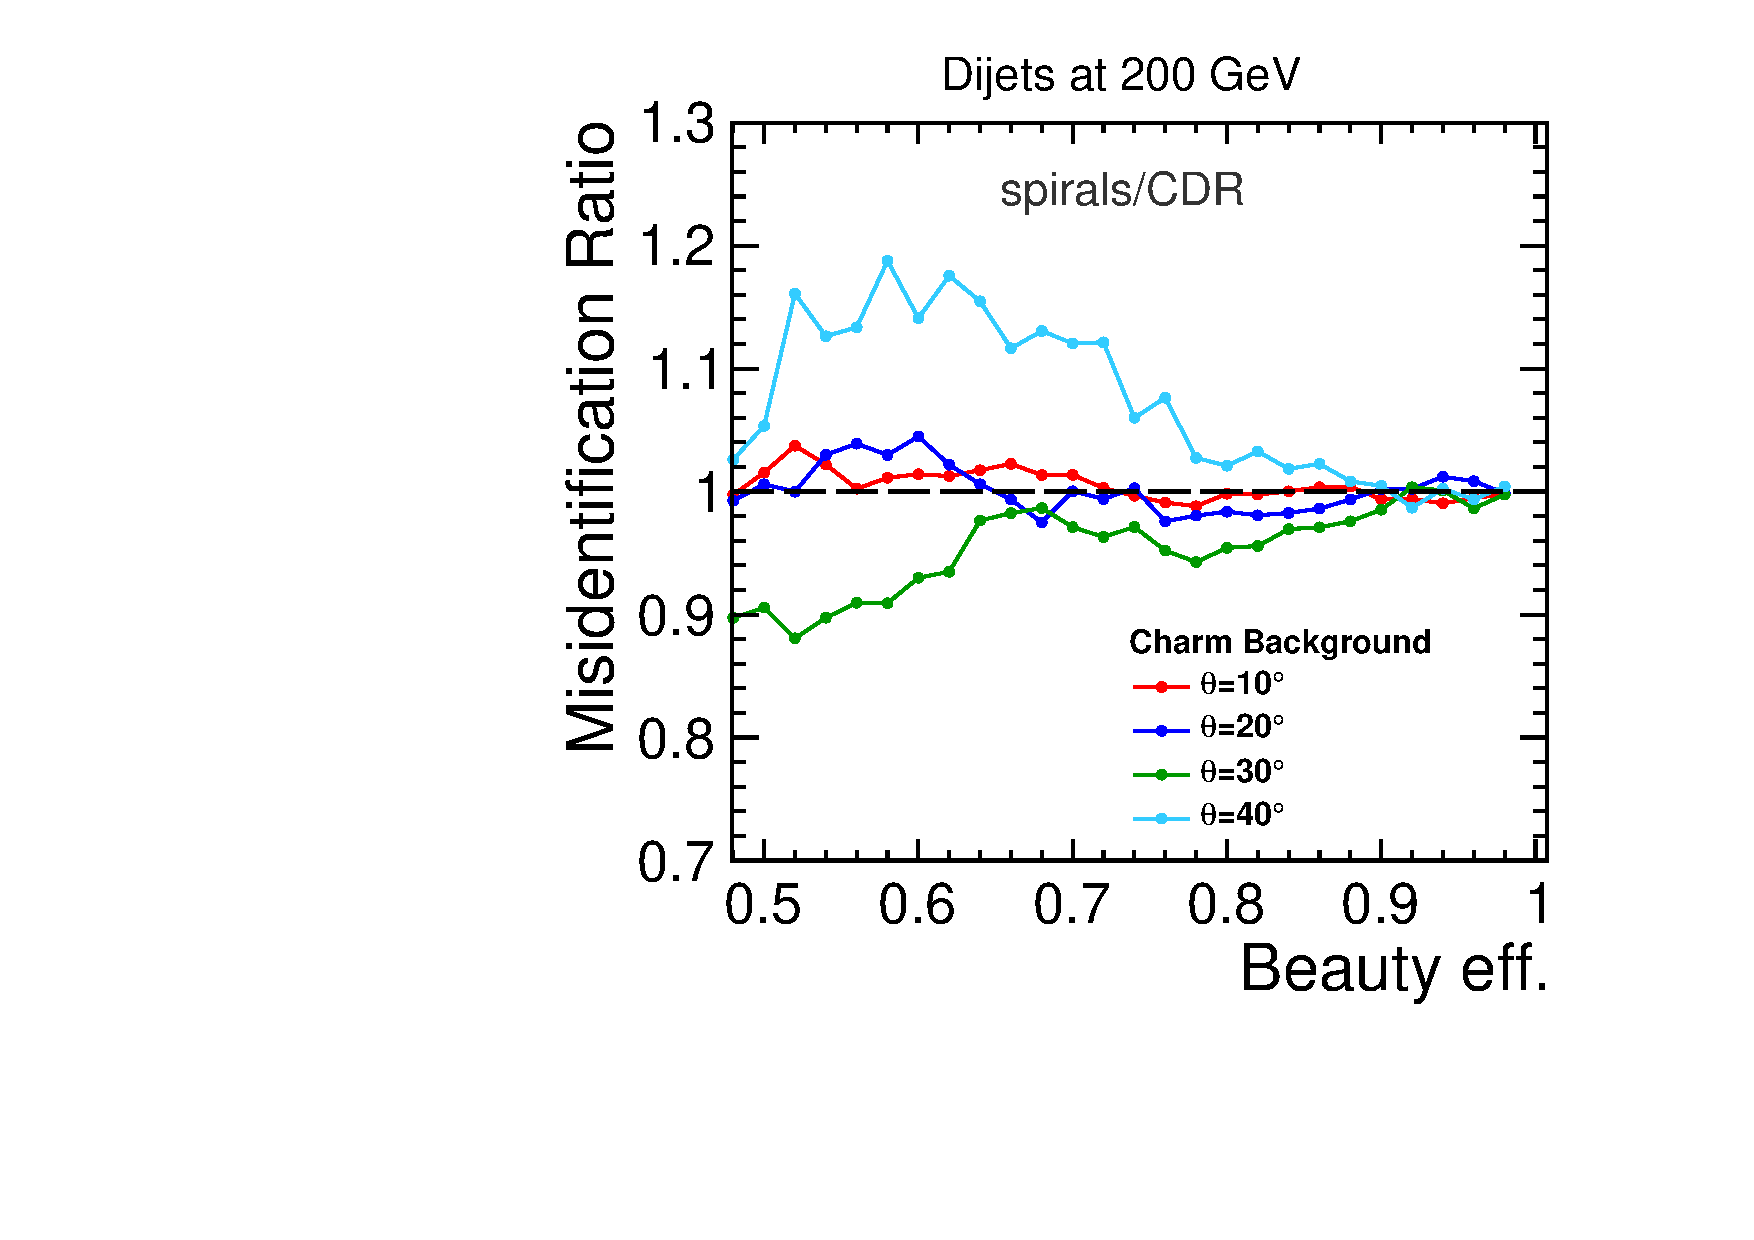
\includegraphics[width=\textwidth]{Figures/ImpactOfGeometries/200GeV_Ratio_allAngles_spirals_CDR_B_C.pdf}};
      \draw[white, fill=white] (1.8, 6.3) rectangle (5.7, 7);
    \end{tikzpicture}
    \caption{}
    \label{fig:200GeV_Ratio_allAngles_spirals_CDR_B_C.pdf}
  \end{subfigure}%
  ~ 
  \begin{subfigure}[b]{0.5\textwidth}
    \centering
    \begin{tikzpicture}
      \node[anchor=south west,inner sep=0] (image) at (0,0){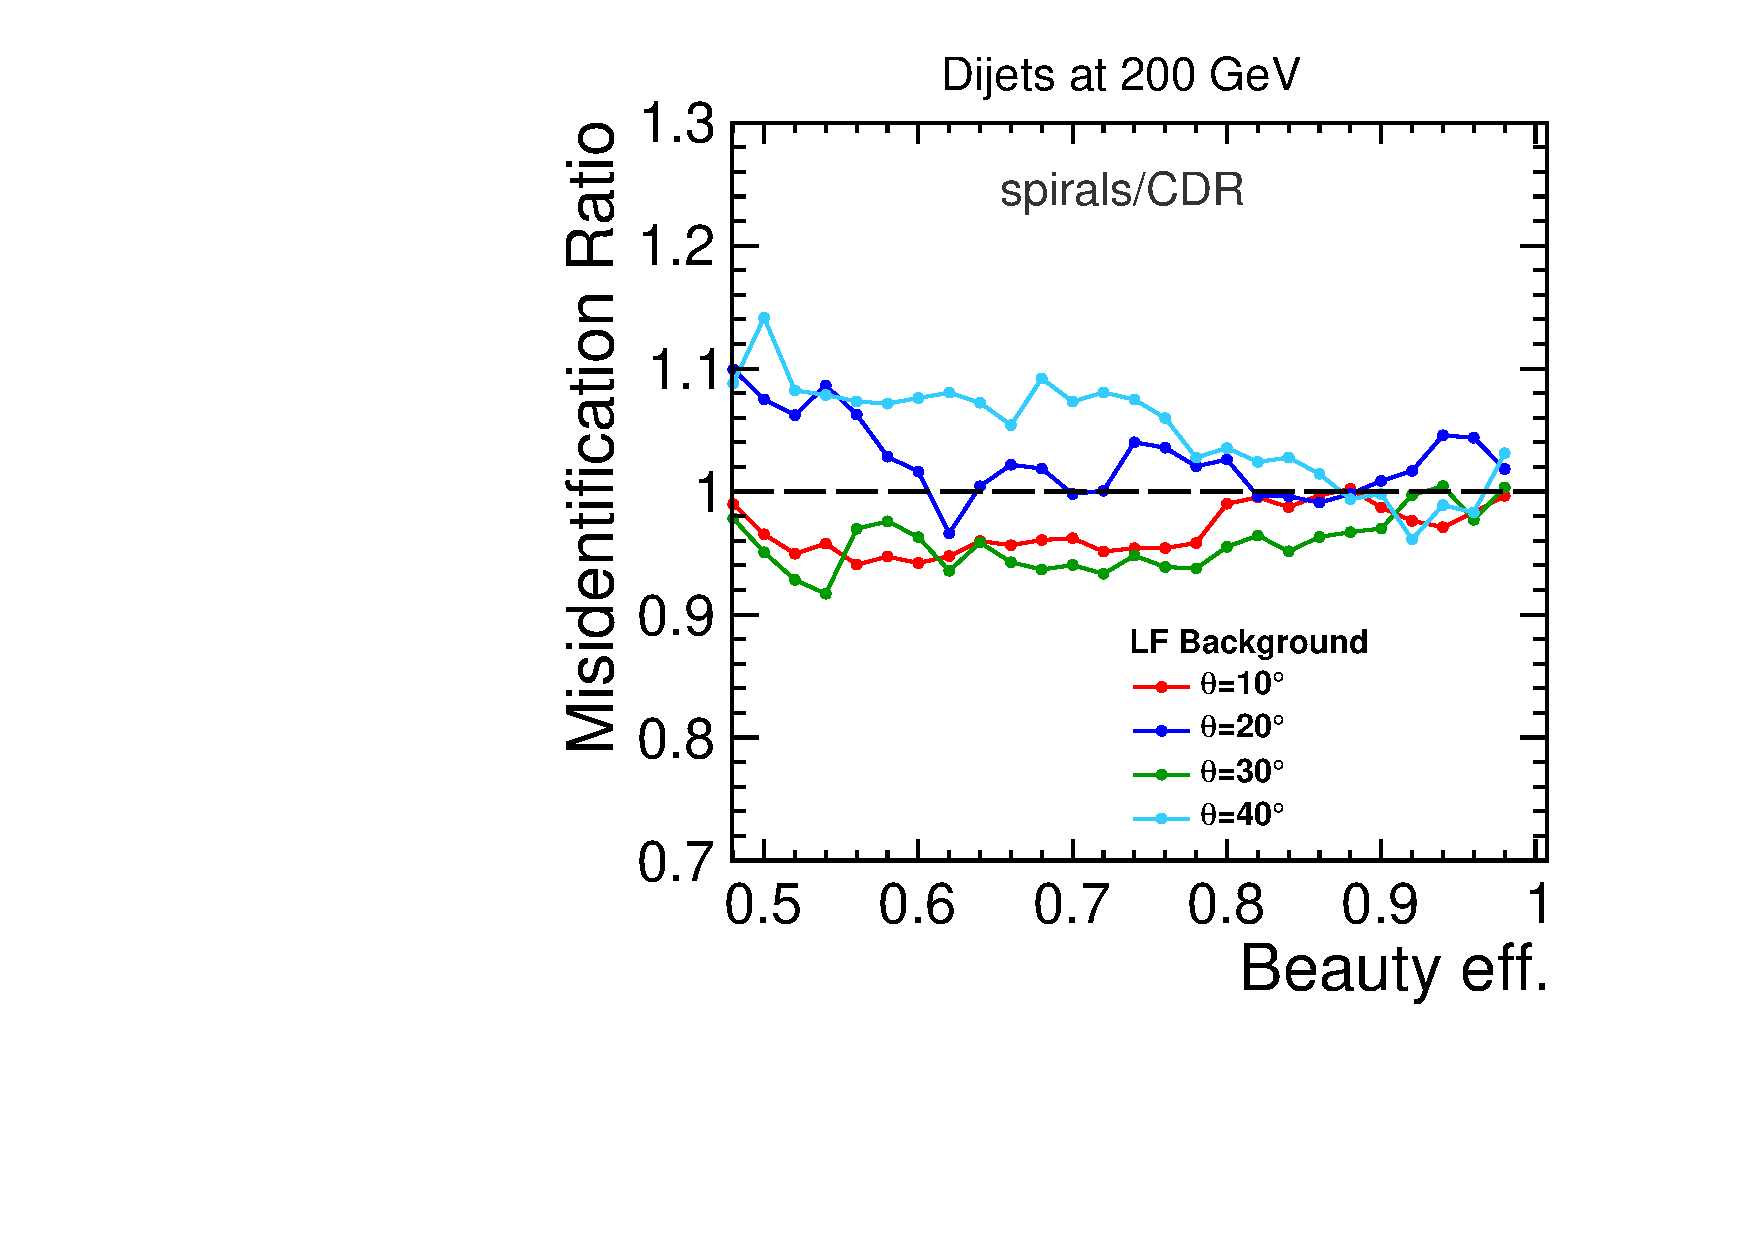
\includegraphics[width=\textwidth]{Figures/ImpactOfGeometries/200GeV_Ratio_allAngles_spirals_CDR_B_LF.pdf}};
      \draw[white, fill=white] (1.8, 6.3) rectangle (5.7, 7);
    \end{tikzpicture}
    \caption{}
    \label{fig:200GeV_Ratio_allAngles_spirals_CDR_B_LF.pdf}
  \end{subfigure}
  \caption{The ratios between the misidentification probabilities for the \textit{spirals} and the CDR geometries as a function of the b-tag efficiency considering the charm (a) and the light flavour (b) backgrounds based on jets in dijet events at $\sqrt{s}=200$~GeV.}\label{fig:spirals_disks_beauty}
\end{figure}

\begin{figure}[H]
  \begin{subfigure}[b]{0.5\textwidth}
    \centering
    \begin{tikzpicture}
      \node[anchor=south west,inner sep=0] (image) at (0,0){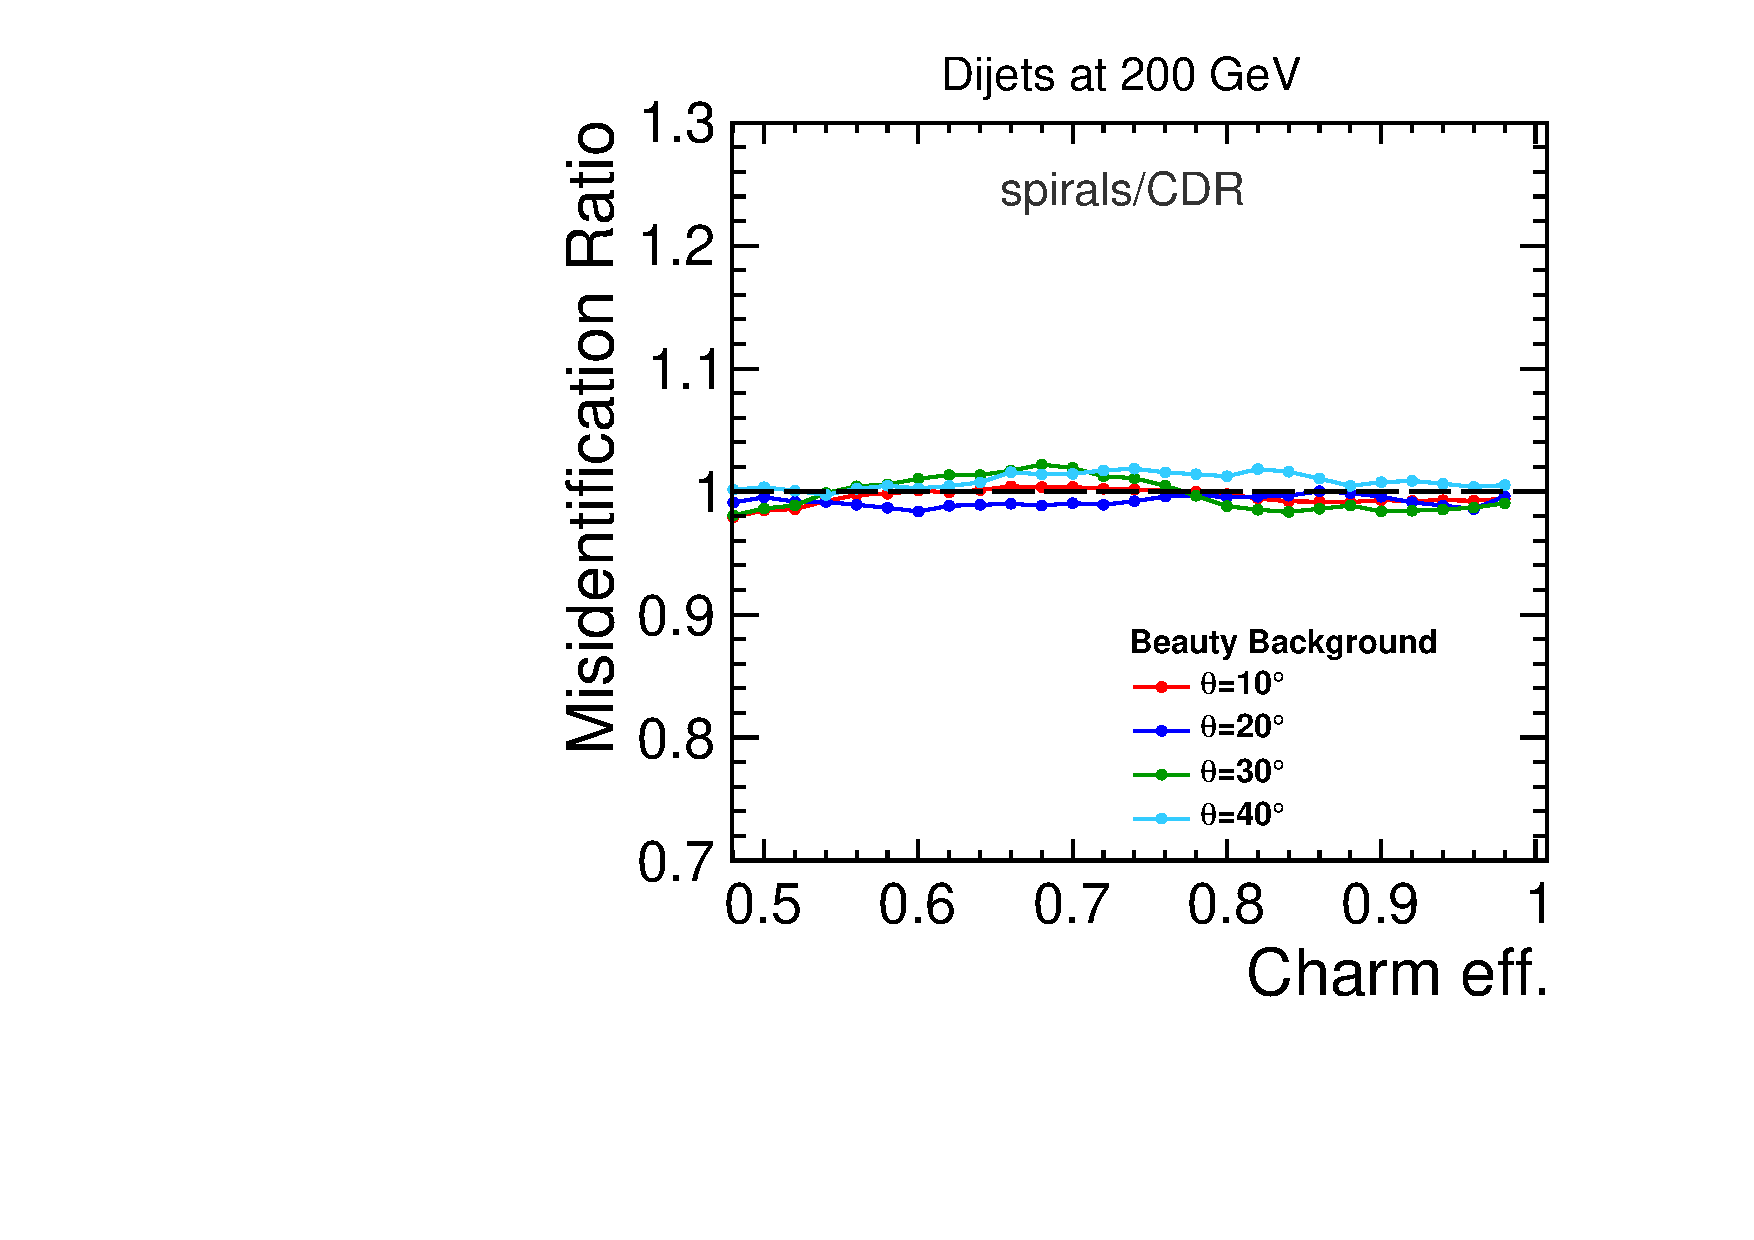
\includegraphics[width=\textwidth]{Figures/ImpactOfGeometries/200GeV_Ratio_allAngles_spirals_CDR_C_B.pdf}};
      \draw[white, fill=white] (1.8, 6.3) rectangle (5.7, 7);
    \end{tikzpicture}
    \caption{}
    \label{ref:200GeV_Ratio_allAngles_spirals_CDR_C_B.pdf}
  \end{subfigure}%
  ~ 
  \begin{subfigure}[b]{0.5\textwidth}
    \centering
    \begin{tikzpicture}
      \node[anchor=south west,inner sep=0] (image) at (0,0){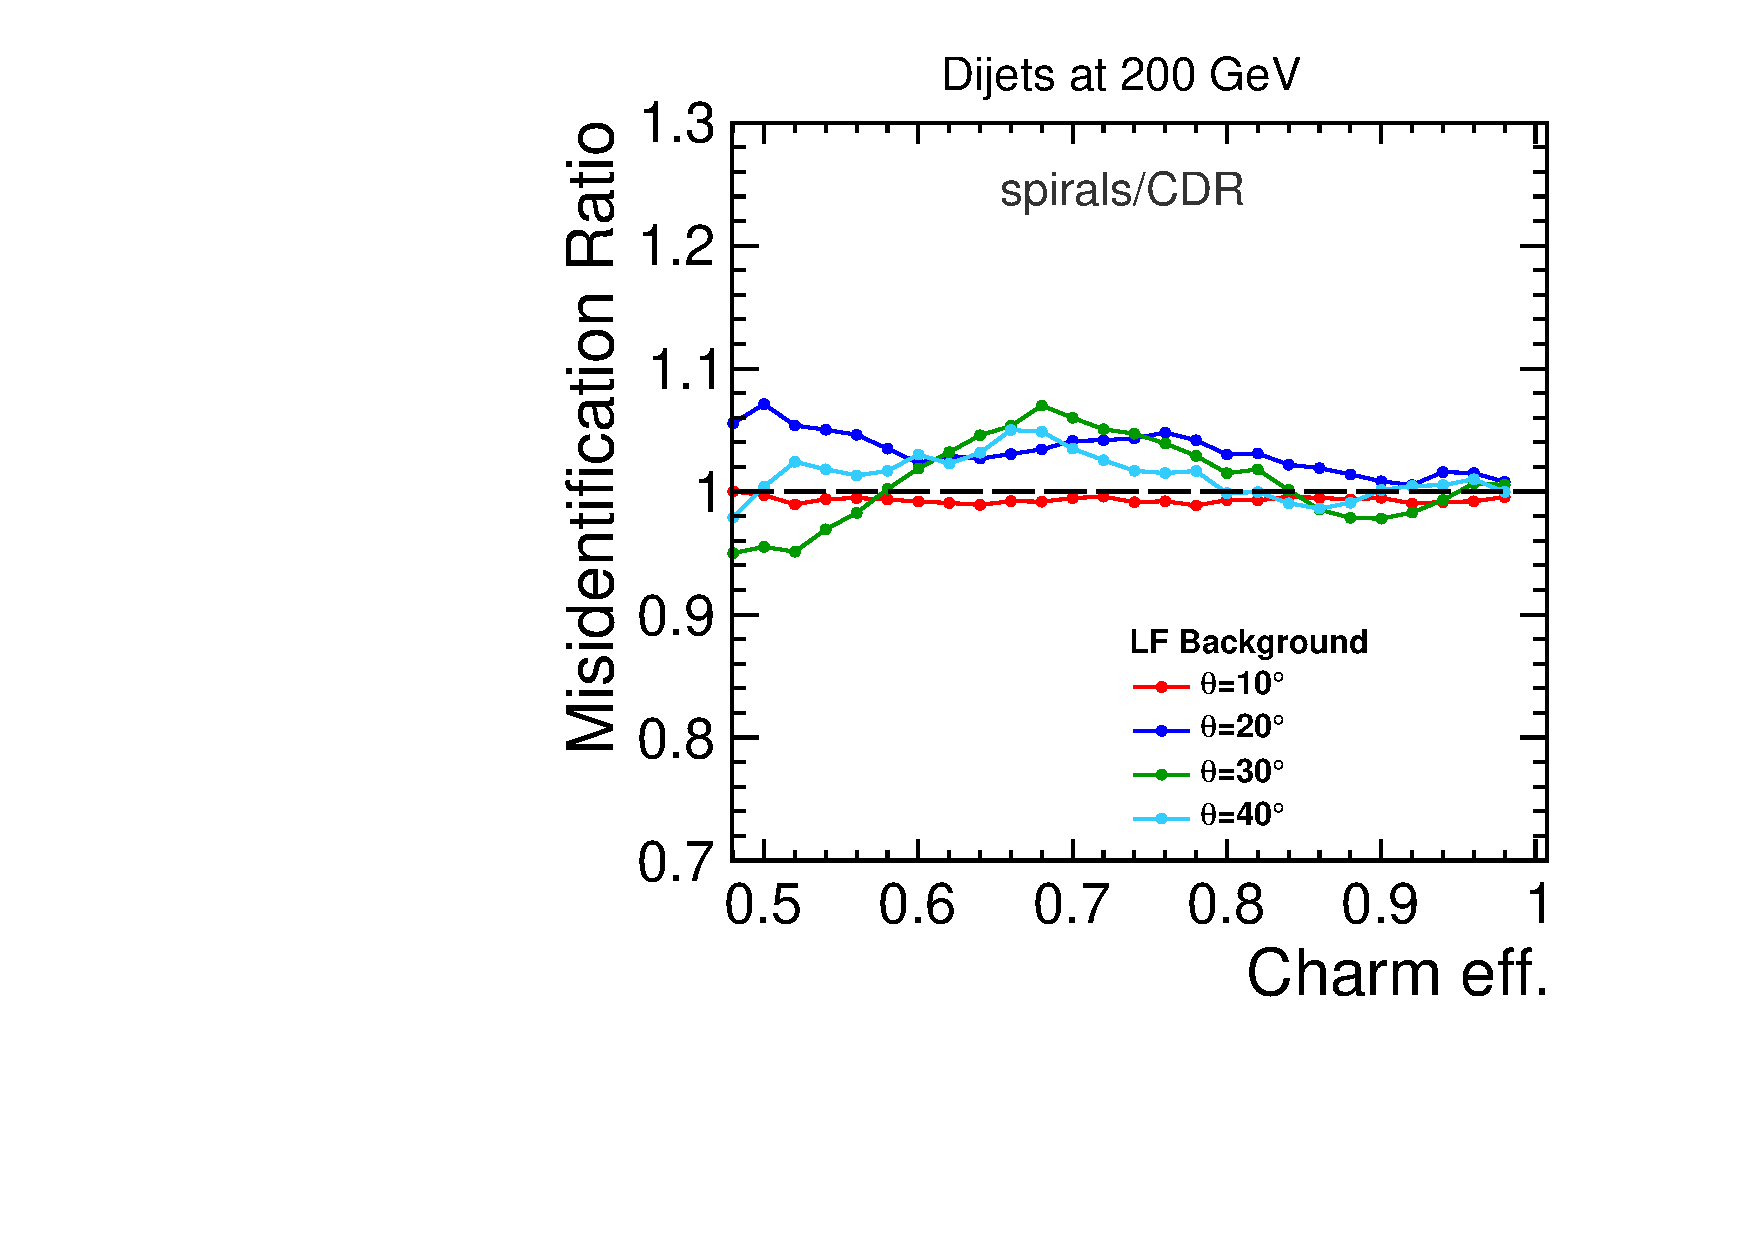
\includegraphics[width=\textwidth]{Figures/ImpactOfGeometries/200GeV_Ratio_allAngles_spirals_CDR_C_LF.pdf}};
      \draw[white, fill=white] (1.8, 6.3) rectangle (5.7, 7);
    \end{tikzpicture}
    \caption{}
    \label{ref:200GeV_Ratio_allAngles_spirals_CDR_C_LF.pdf}
  \end{subfigure}
  \caption{The ratios between the misidentification probabilities for the \textit{spirals} and the CDR geometries as a function of the c-tag efficiency considering the beauty (a) and the light flavour (b) backgrounds based on jets in dijet events at $\sqrt{s}=200$~GeV.}\label{fig:spirals_disks_charm}
\end{figure}


%----------------------------------------------------------------------
\subsubsection{\emph{double\_spirals} and \emph{spirals}}

The \begin{it}double\_spirals\end{it} and the \textit{spirals} geometries are compared using dijet events with a mixture of polar angles between $10^{\circ}$ and $90^{\circ}$. For each jet flavour, 720000 events are included (for each $\theta$ value, the same number of events is used). Having large number of events allows to reduce the statistical fluctuations.\\
The comparison between the two geometries is shown in Figures \ref{fig:globalComparison_double_spirals_1000}, \ref{fig:globalComparison_double_spirals_500}, \ref{fig:globalComparison_double_spirals_200} and \ref{fig:globalComparison_double_spirals_91}. The performances of these two geometries are similar.\\ 
For jets in dijet events at $\sqrt{s}=$1000~GeV, the \textit{double\_spirals} geometry shows a better performance for beauty and charm tagging. For jets in dijet events at $\sqrt{s}=$500~GeV and $\sqrt{s}=$200~GeV, the ratio between the misidentification probabilities varies between $\pm 10\%$. For jets in dijet events at $\sqrt{s}=$91~GeV, the c-tag performance shows better results for light-flavour rejection with the \textit{double\_spirals} geometry. This effect might be explained by the fact that double-sided modules provide two measurements which are close to the interaction point and improve the track reconstruction. In some cases, it is possible that the B hadron decays after the first layer in the vertex barrel. In the CDR and the \textit{spirals} geometry, one measurement layer is lost. With the \textit{double\_spirals} configuration, two measurement layers are lost. But in total, the number of hits is identical if the decay of the B hadrons occurs after the first layer for the three geometries.\\
More results for different jet energies and angles can be found in Appendix~\ref{sec:appendix_doubleSpirals_vs_spirals}.

\begin{figure}[H]
  \begin{subfigure}[b]{0.5\textwidth}
    \centering
    \begin{tikzpicture}
      \node[anchor=south west,inner sep=0] (image) at (0,0){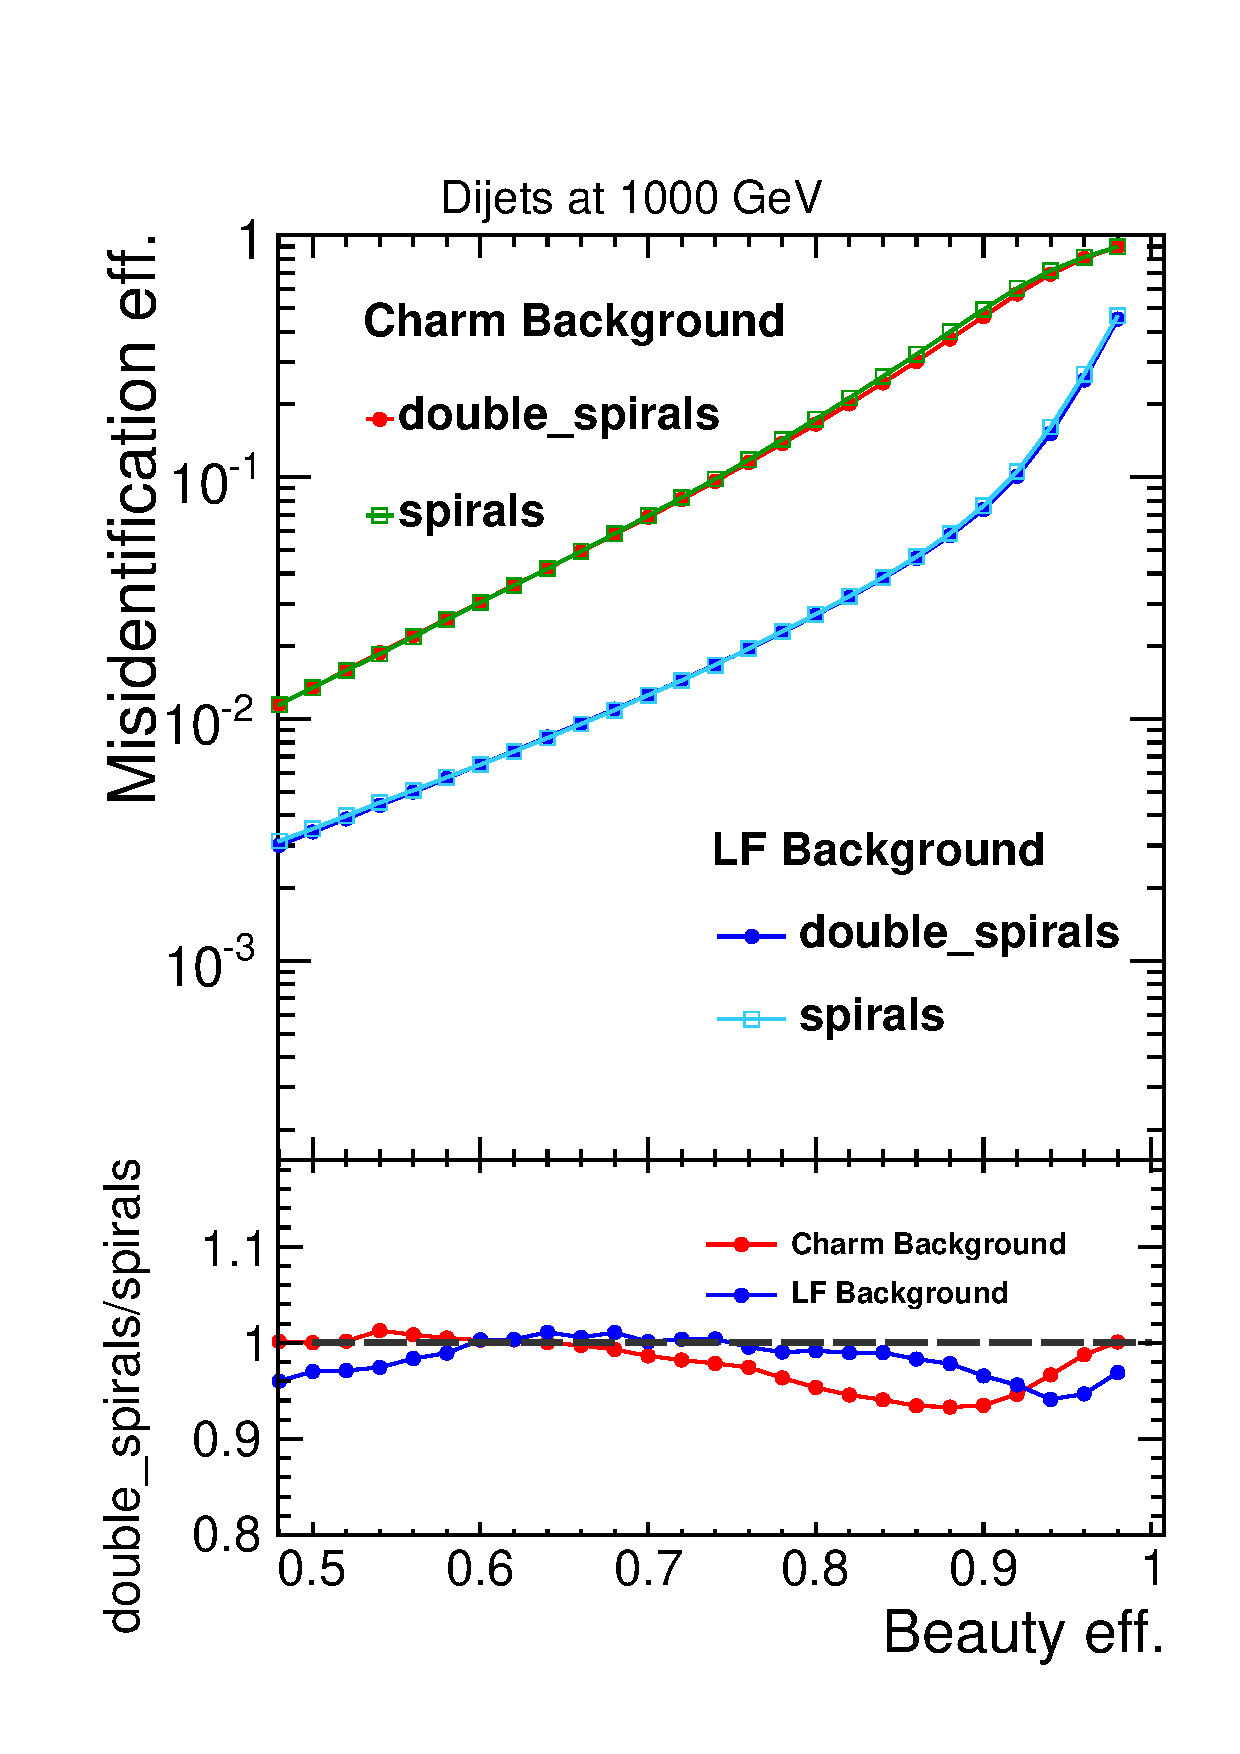
\includegraphics[width=\textwidth]{Figures/ImpactOfGeometries/general_1000_Beauty.pdf}};
      \draw[white, fill=white] (1.8, 9.95) rectangle (5.5, 10.6);
    \end{tikzpicture}
    \caption{}
    \label{}
  \end{subfigure}%
  ~ 
  \begin{subfigure}[b]{0.5\textwidth}
    \centering
    \begin{tikzpicture}
      \node[anchor=south west,inner sep=0] (image) at (0,0){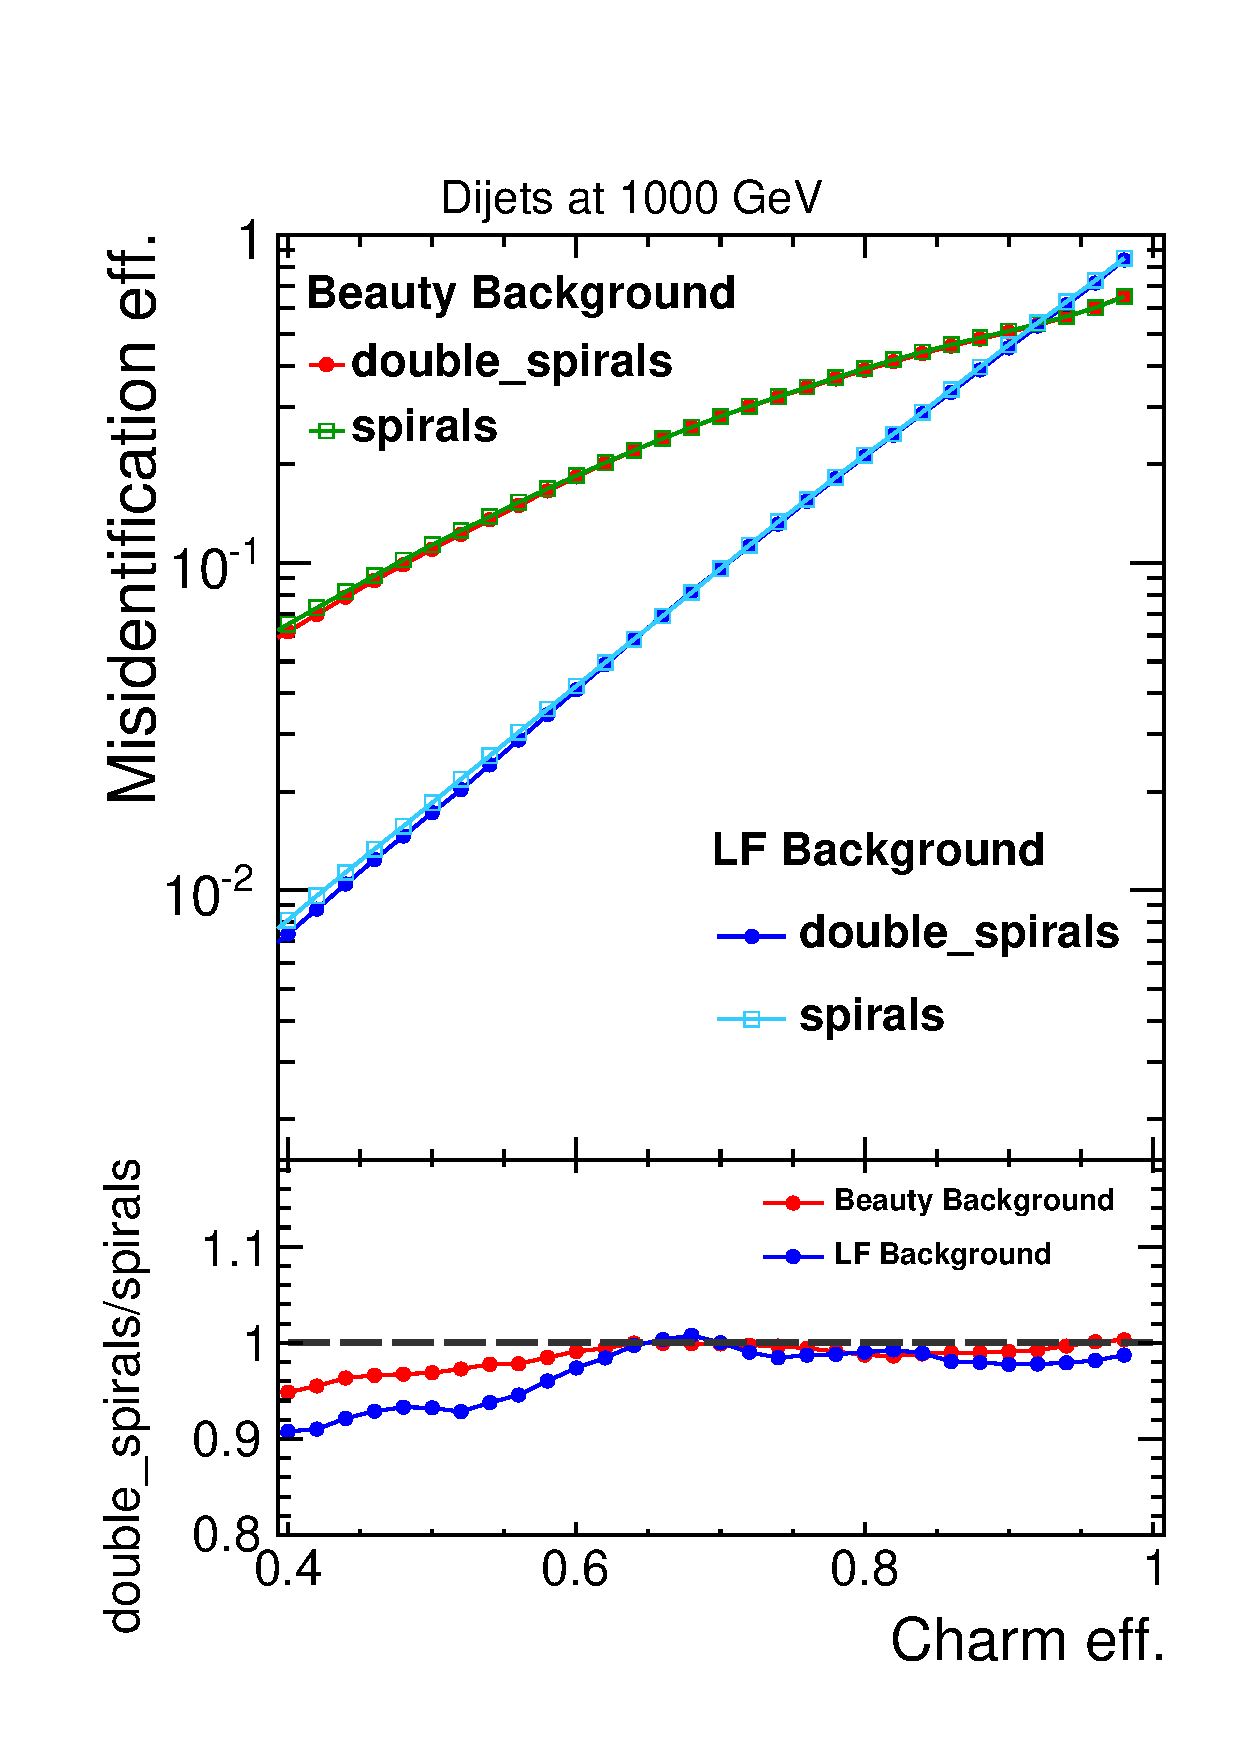
\includegraphics[width=\textwidth]{Figures/ImpactOfGeometries/general_1000_Charm.pdf}};
      \draw[white, fill=white] (1.8, 9.95) rectangle (5.5, 10.6);
    \end{tikzpicture}
    \caption{}
    \label{}
  \end{subfigure}
  \caption{Global comparison between the \textit{double\_spirals} and the
    \textit{spirals} geometries based on beauty tagging (a) and charm
    tagging (b) for jets in dijet events at $\sqrt{s}=$1000~GeV with a
    mixture of polar angles between $10^{\circ}$ and $90^{\circ}$. On the y-axis, the misidentification probability and the ratio between the misidentification probabilities for the two geometries are given.}\label{fig:globalComparison_double_spirals_1000}
\end{figure}

\begin{figure}[H]
  \begin{subfigure}[b]{0.5\textwidth}
    \centering
    \begin{tikzpicture}
      \node[anchor=south west,inner sep=0] (image) at (0,0){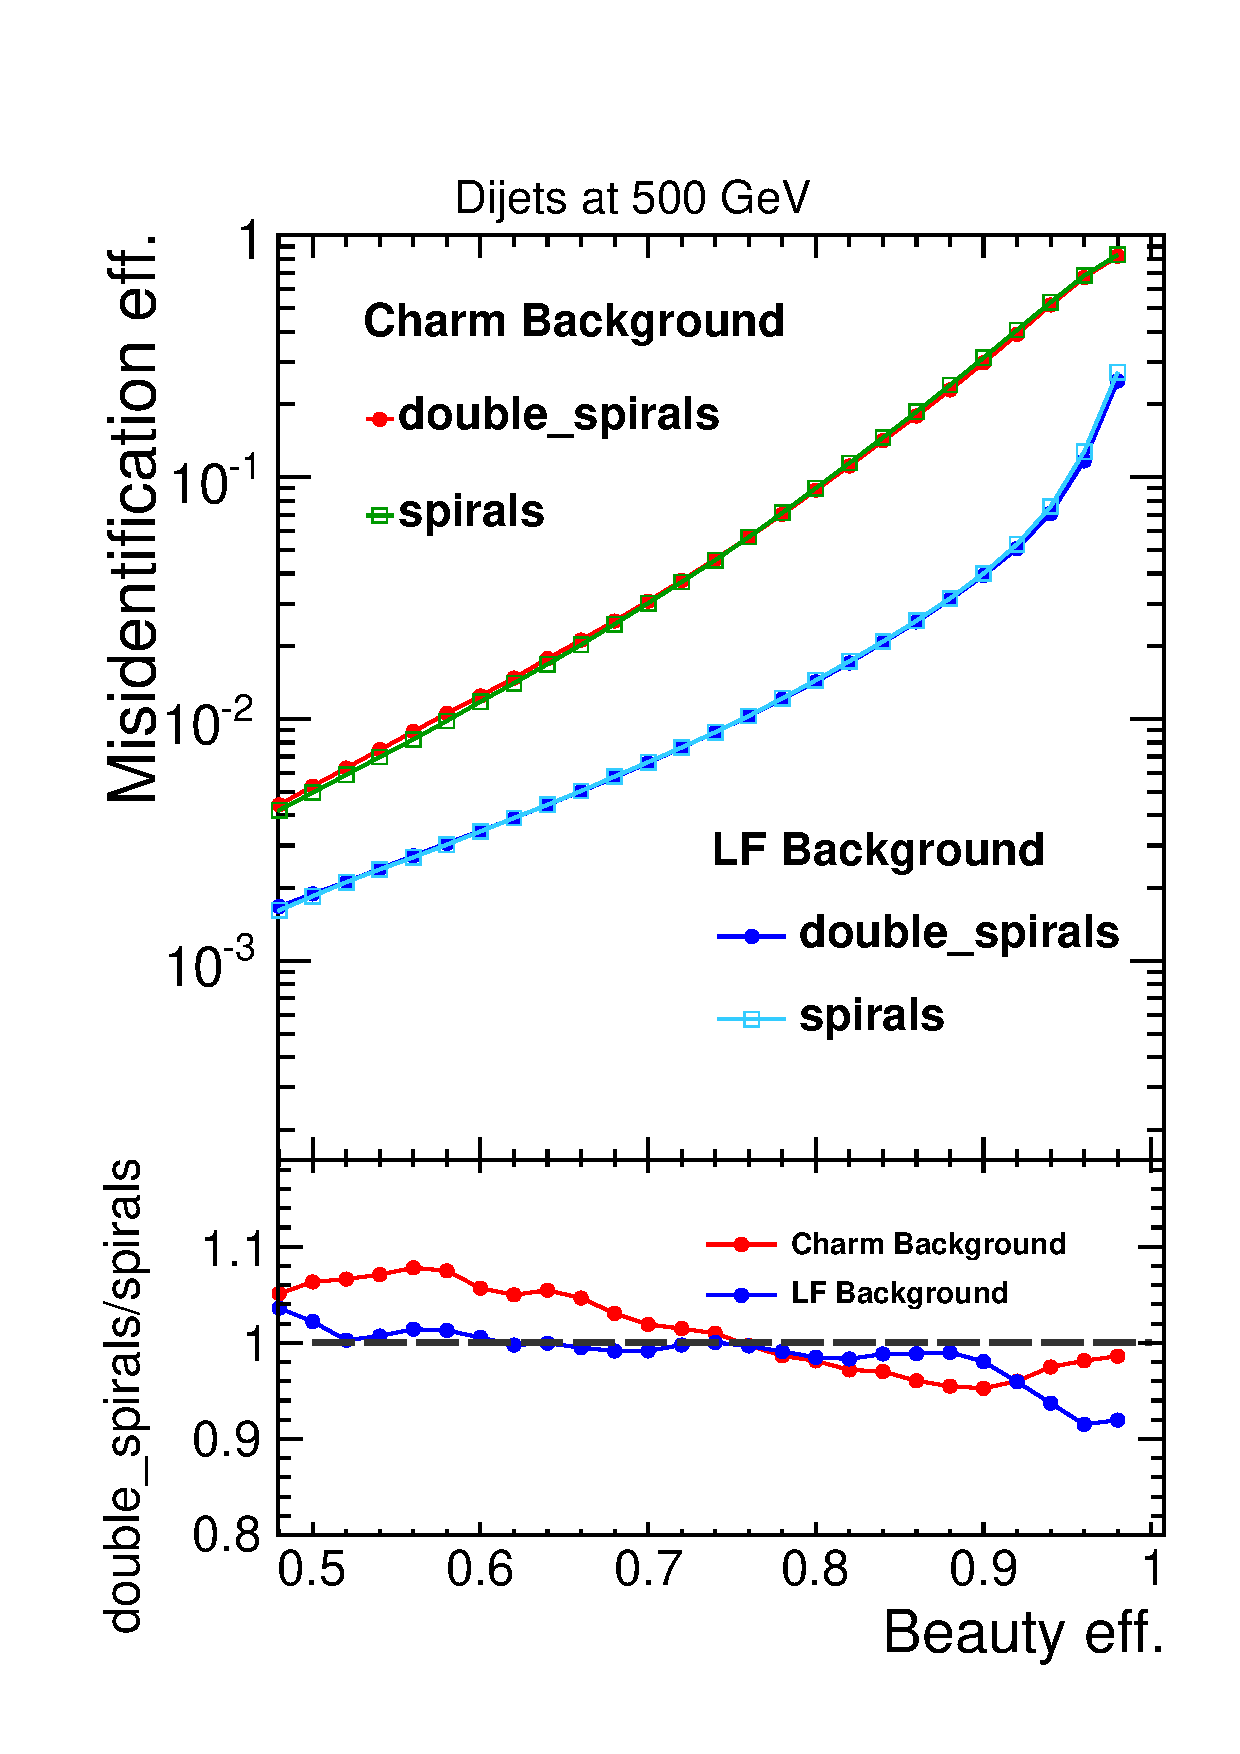
\includegraphics[width=\textwidth]{Figures/ImpactOfGeometries/general_500_Beauty.pdf}};
      \draw[white, fill=white] (1.8, 9.95) rectangle (5.5, 10.6);
    \end{tikzpicture}
    \caption{}
    \label{}
  \end{subfigure}%
  ~ 
  \begin{subfigure}[b]{0.5\textwidth}
    \centering
        \begin{tikzpicture}
      \node[anchor=south west,inner sep=0] (image) at (0,0){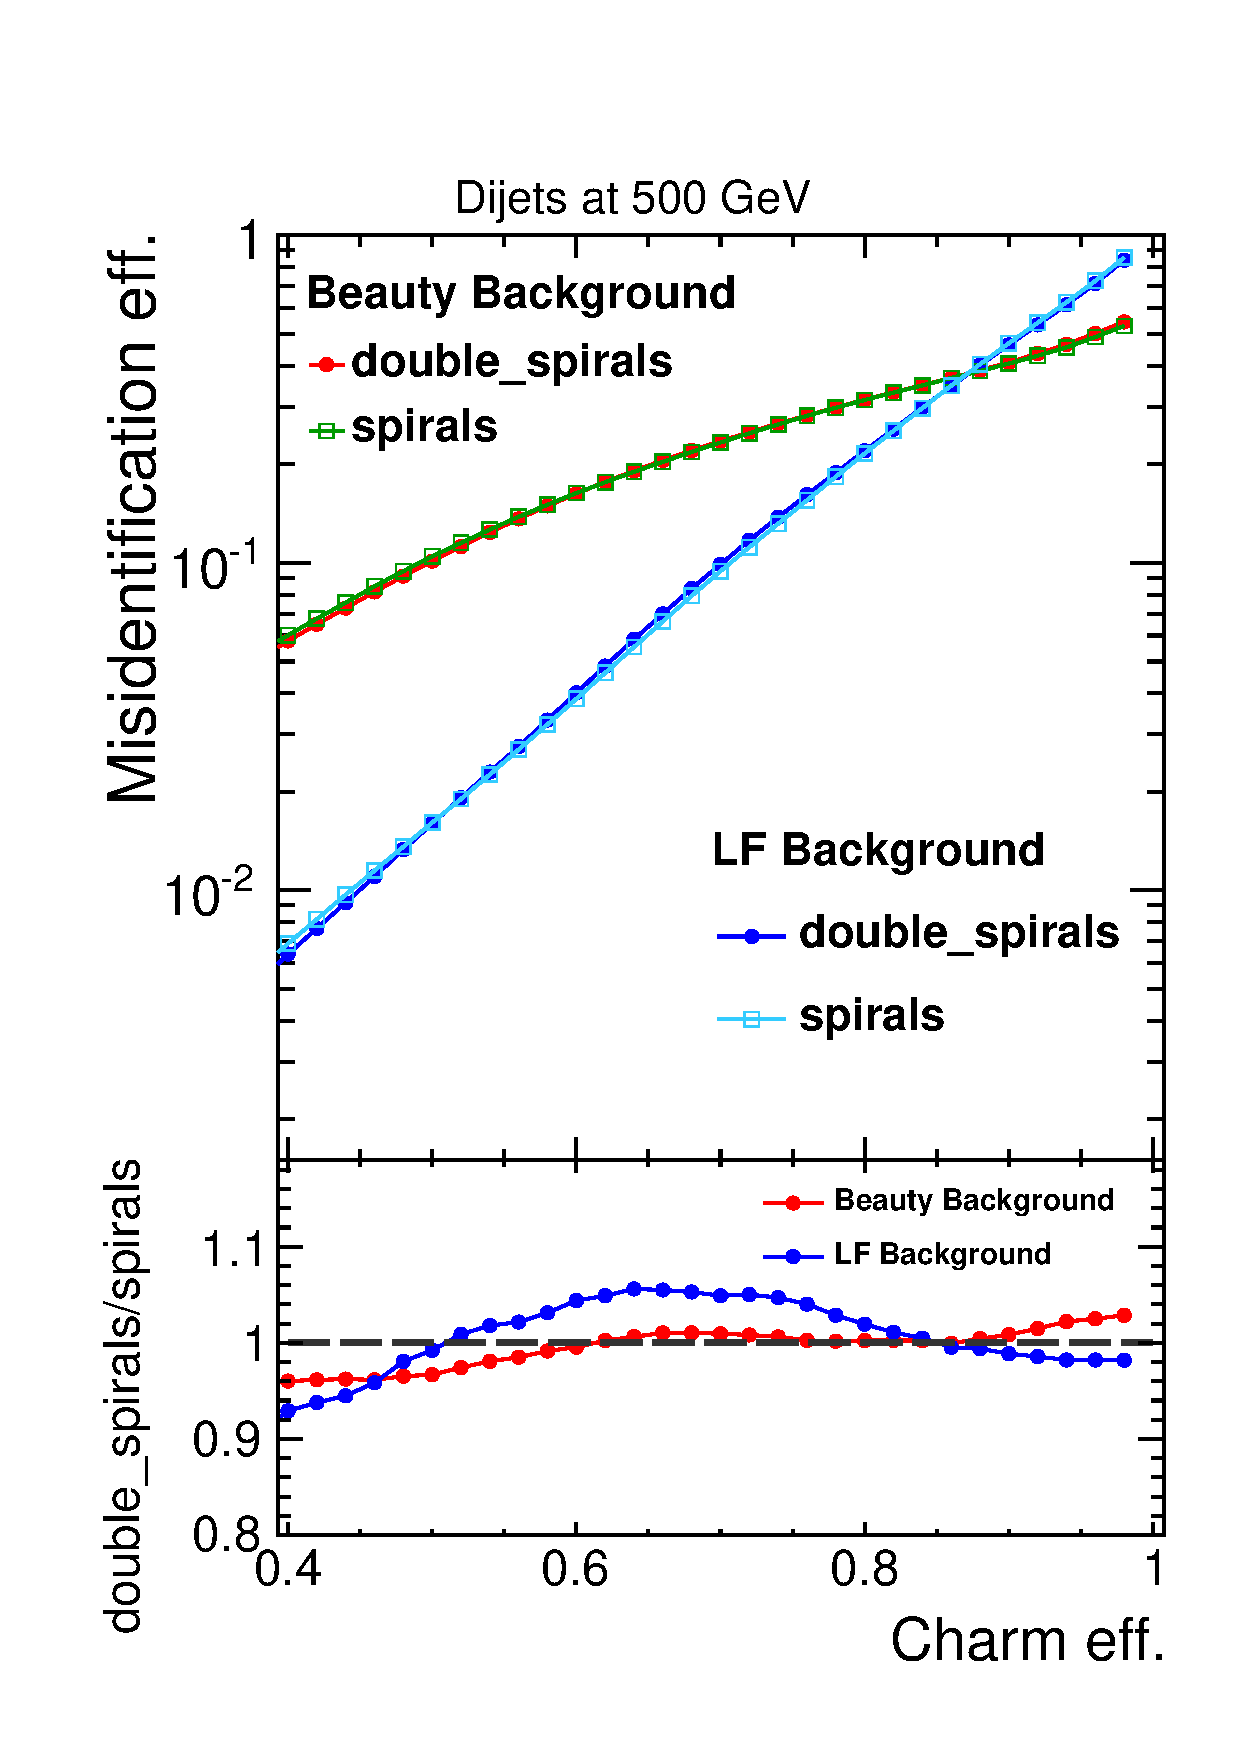
\includegraphics[width=\textwidth]{Figures/ImpactOfGeometries/general_500_Charm.pdf}};
      \draw[white, fill=white] (1.8, 9.95) rectangle (5.5, 10.6);
        \end{tikzpicture}
        \caption{}
        \label{}
  \end{subfigure}
  \caption{Global comparison between the \textit{double\_spirals} and the
    \textit{spirals} geometries based on beauty tagging (a) and charm
    tagging (b) for jets in dijet events at $\sqrt{s}=$500~GeV with a mixture of polar
    angles between $10^{\circ}$ and $90^{\circ}$. On the y-axis, the misidentification probability and the ratio between the misidentification probabilities for the two geometries are given.}\label{fig:globalComparison_double_spirals_500}
\end{figure}

\begin{figure}[H]
  \begin{subfigure}[b]{0.5\textwidth}
    \centering
    \begin{tikzpicture}
      \node[anchor=south west,inner sep=0] (image) at (0,0){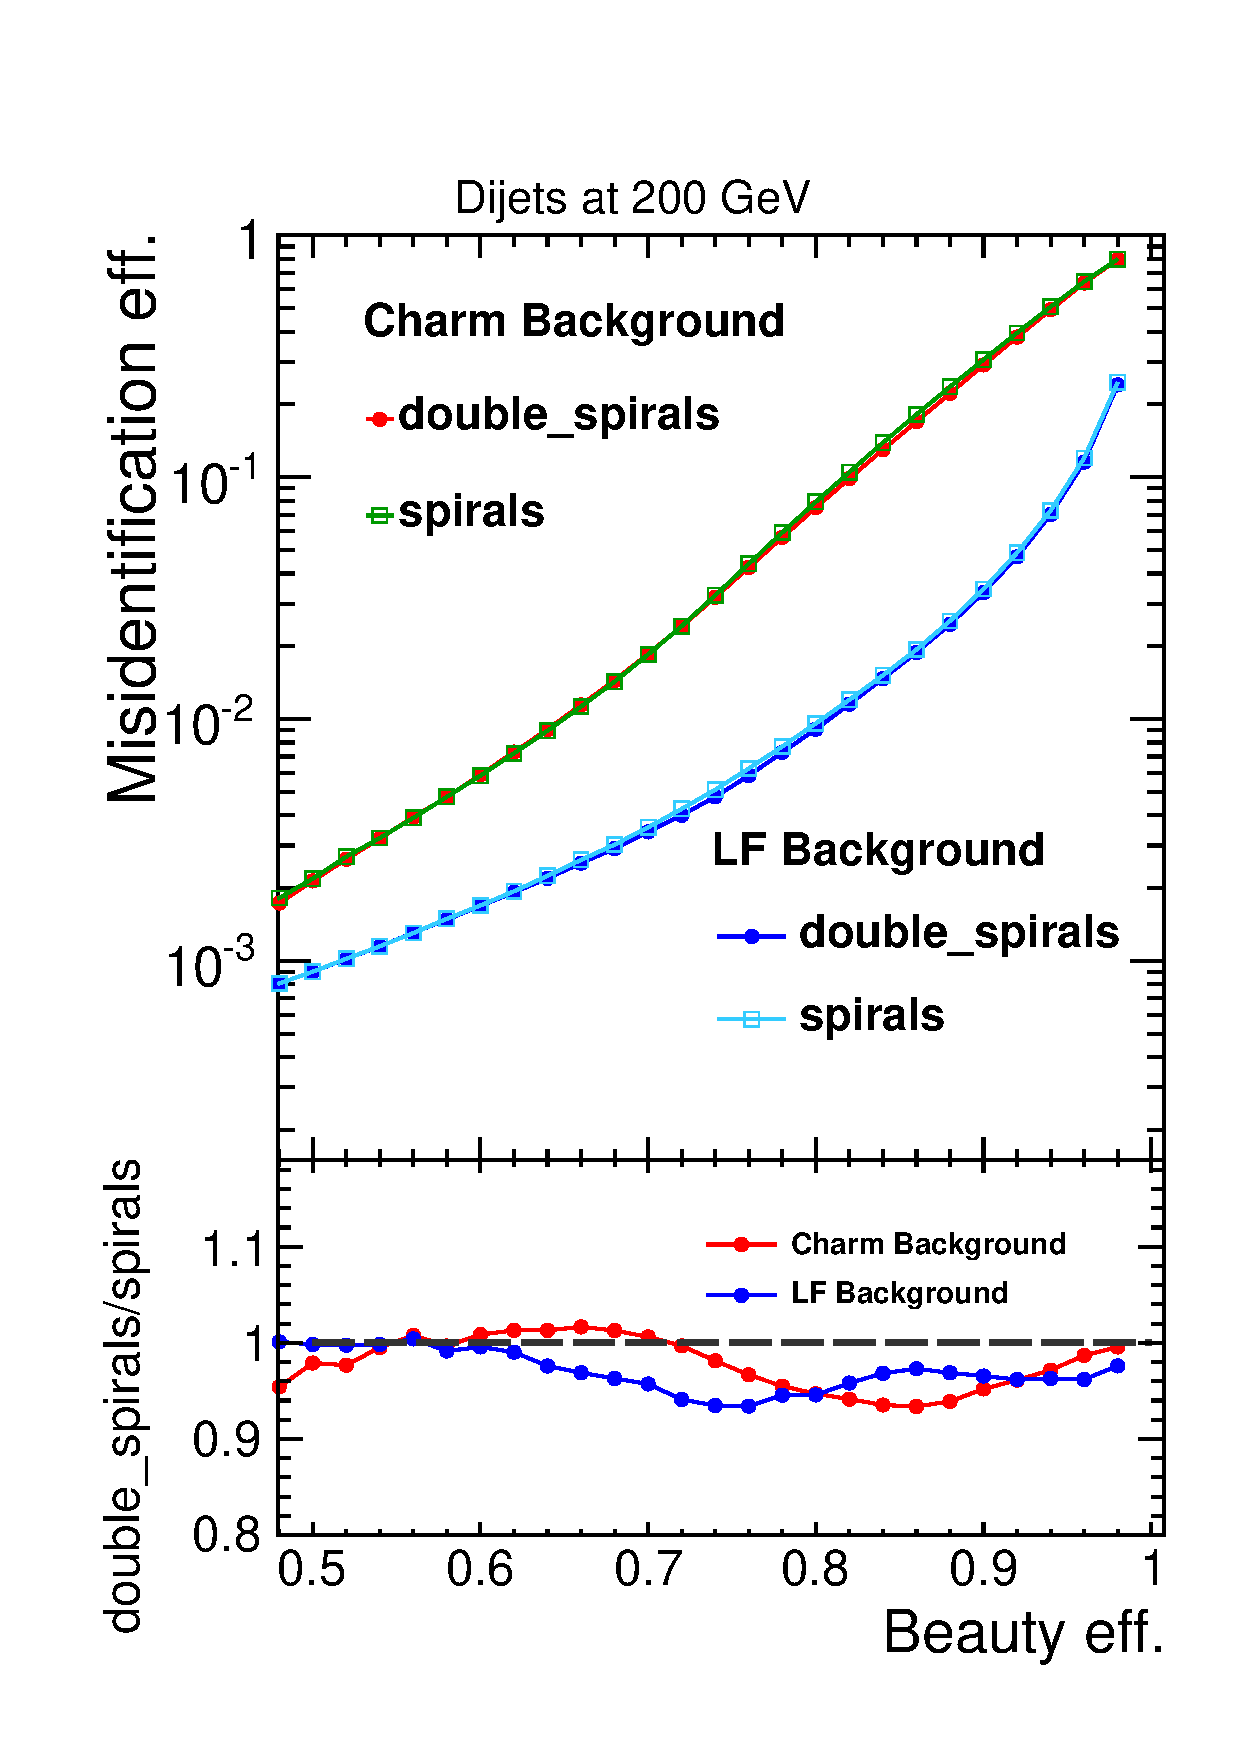
\includegraphics[width=\textwidth]{Figures/ImpactOfGeometries/general_200_Beauty.pdf}};
      \draw[white, fill=white] (1.8, 9.95) rectangle (5.5, 10.6);
    \end{tikzpicture}
    \caption{}
    \label{}
  \end{subfigure}%
  ~ 
  \begin{subfigure}[b]{0.5\textwidth}
    \centering
    \begin{tikzpicture}
      \node[anchor=south west,inner sep=0] (image) at (0,0){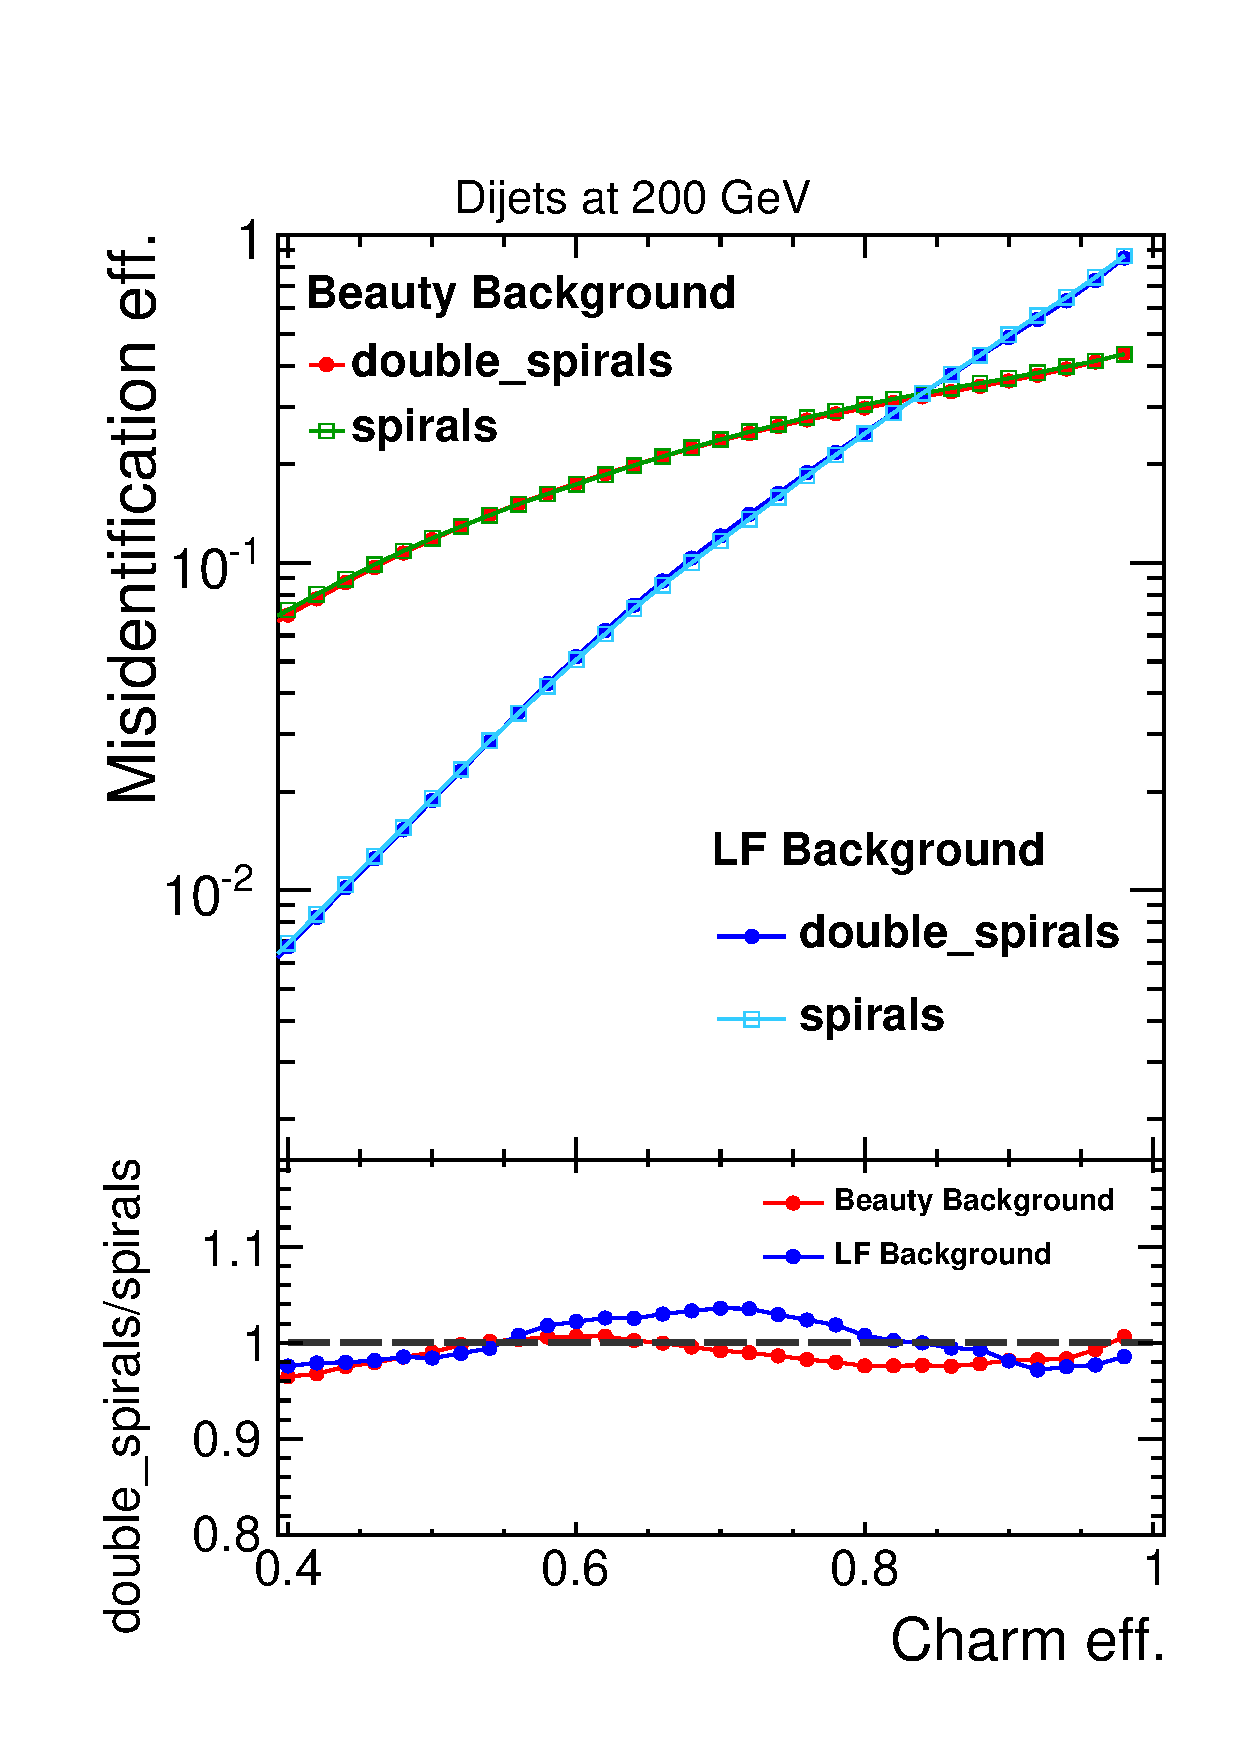
\includegraphics[width=\textwidth]{Figures/ImpactOfGeometries/general_200_Charm.pdf}};
      \draw[white, fill=white] (1.8, 9.95) rectangle (5.5, 10.6);
    \end{tikzpicture}
    \caption{}
    \label{}
  \end{subfigure}
  \caption{Global comparison between the \textit{double\_spirals} and the \textit{spirals} geometries based on beauty tagging (a) and charm
    tagging (b) for jets in dijet events at $\sqrt{s}=$200~GeV with a mixture of polar
    angles between $10^{\circ}$ and $90^{\circ}$. On the y-axis, the misidentification probability and the ratio between the misidentification probabilities for the two geometries are given.}\label{fig:globalComparison_double_spirals_200}
\end{figure}

\begin{figure}[H]
  \begin{subfigure}[b]{0.5\textwidth}
    \centering
    \begin{tikzpicture}
      \node[anchor=south west,inner sep=0] (image) at (0,0){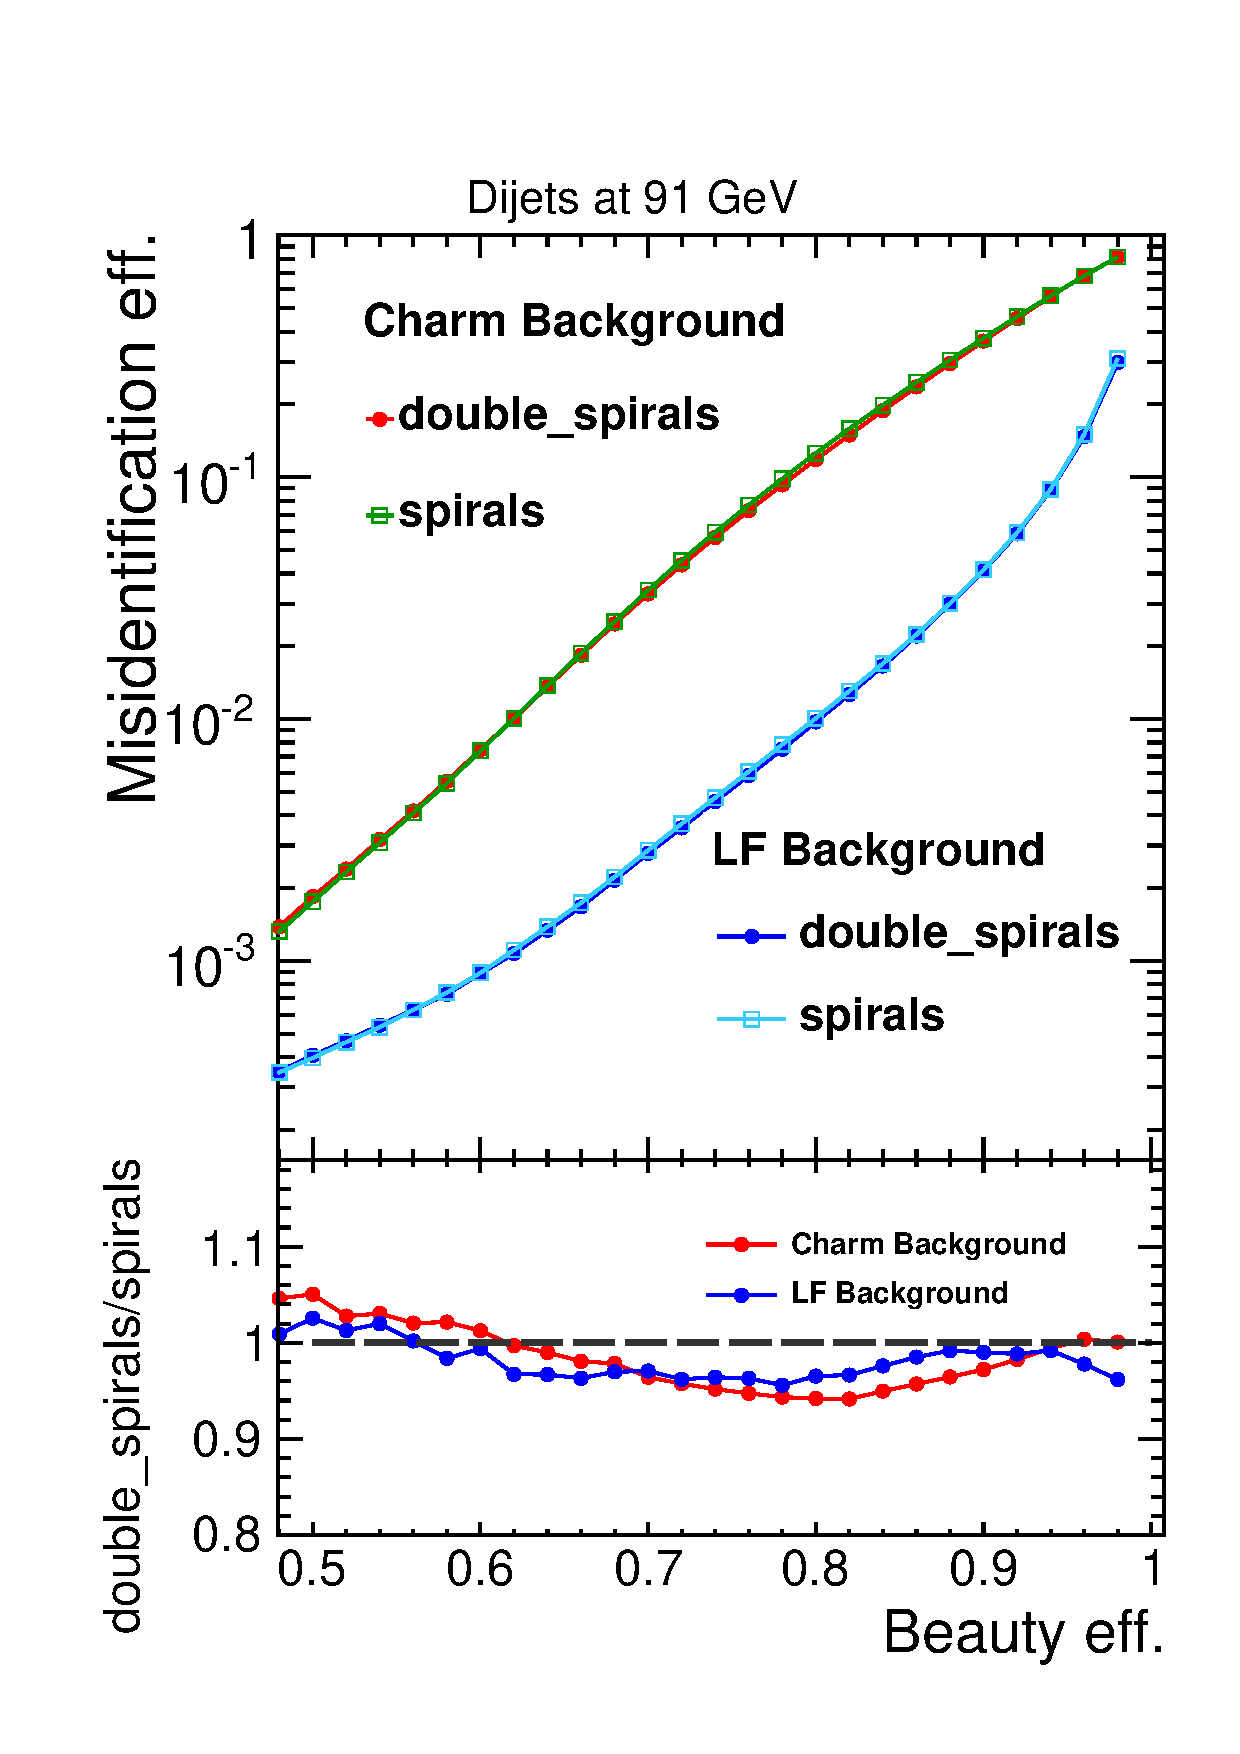
\includegraphics[width=\textwidth]{Figures/ImpactOfGeometries/general_91_Beauty.pdf}};
      \draw[white, fill=white] (1.8, 9.95) rectangle (5.5, 10.6);
    \end{tikzpicture}
    \caption{}
    \label{}
  \end{subfigure}%
  ~ 
  \begin{subfigure}[b]{0.5\textwidth}
    \centering
    \begin{tikzpicture}
      \node[anchor=south west,inner sep=0] (image) at (0,0){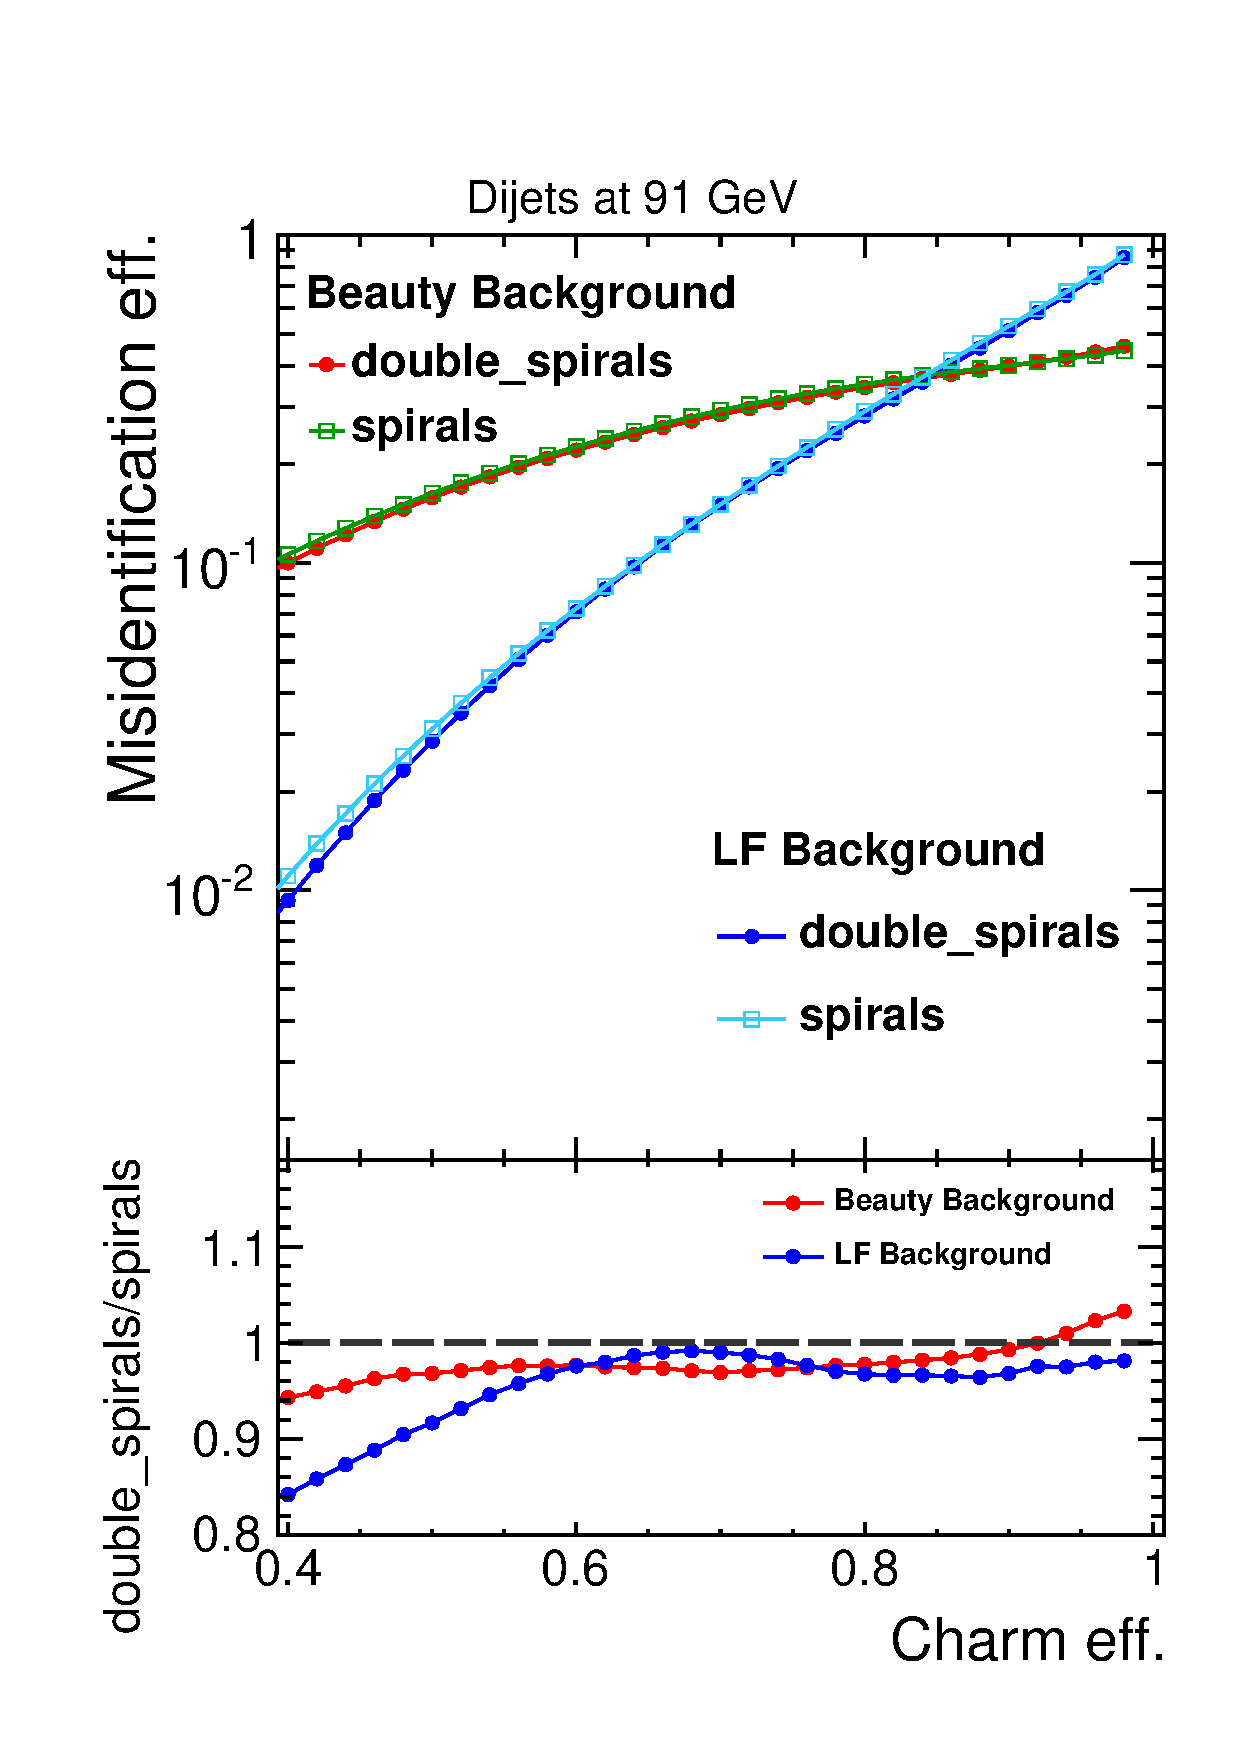
\includegraphics[width=\textwidth]{Figures/ImpactOfGeometries/general_91_Charm.pdf}};
      \draw[white, fill=white] (1.8, 9.95) rectangle (5.5, 10.6);
    \end{tikzpicture}
    \caption{}
    \label{}
  \end{subfigure}
  \caption{Global comparison between the \textit{double\_spirals} and the
    \textit{spirals} geometries based on beauty tagging (a) and charm
    tagging (b) for jets in dijet events at $\sqrt{s}=$91~GeV with a
    mixture of polar angles between $10^{\circ}$ and $90^{\circ}$. On the y-axis, the misidentification probability and the ratio between the misidentification probabilities for the two geometries are given.}\label{fig:globalComparison_double_spirals_91}
\end{figure}


%----------------------------------------------------------------------
\subsubsection{\emph{double\_spirals} and CDR}
The comparison between the \textit{double\_spirals} and the CDR geometries is given in Figures \ref{fig:double_disks_beauty} and \ref{fig:double_disks_charm}. \\
In general, the performance of the two geometries is very similar except for dijet events at $\theta=40^\circ$ where the b-tagging performance for the \textit{double\_spirals} geometry decreases by up to 30\% (the same effect is also observed when comparing the \textit{spirals} and the CDR geometries in Section \ref{sec:spirals_CDR}). This polar angle falls in the transition region between the vertex endcaps and barrel. The same effect is discussed in Section~\ref{sec:spirals_CDR}. \\
More results for different jet energies can be found in Appendix~\ref{sec:appendix_doubleSpirals_vs_CDR}.

\begin{figure}[H]
  \begin{subfigure}[b]{0.5\textwidth}
    \centering
    \begin{tikzpicture}
      \node[anchor=south west,inner sep=0] (image) at (0,0){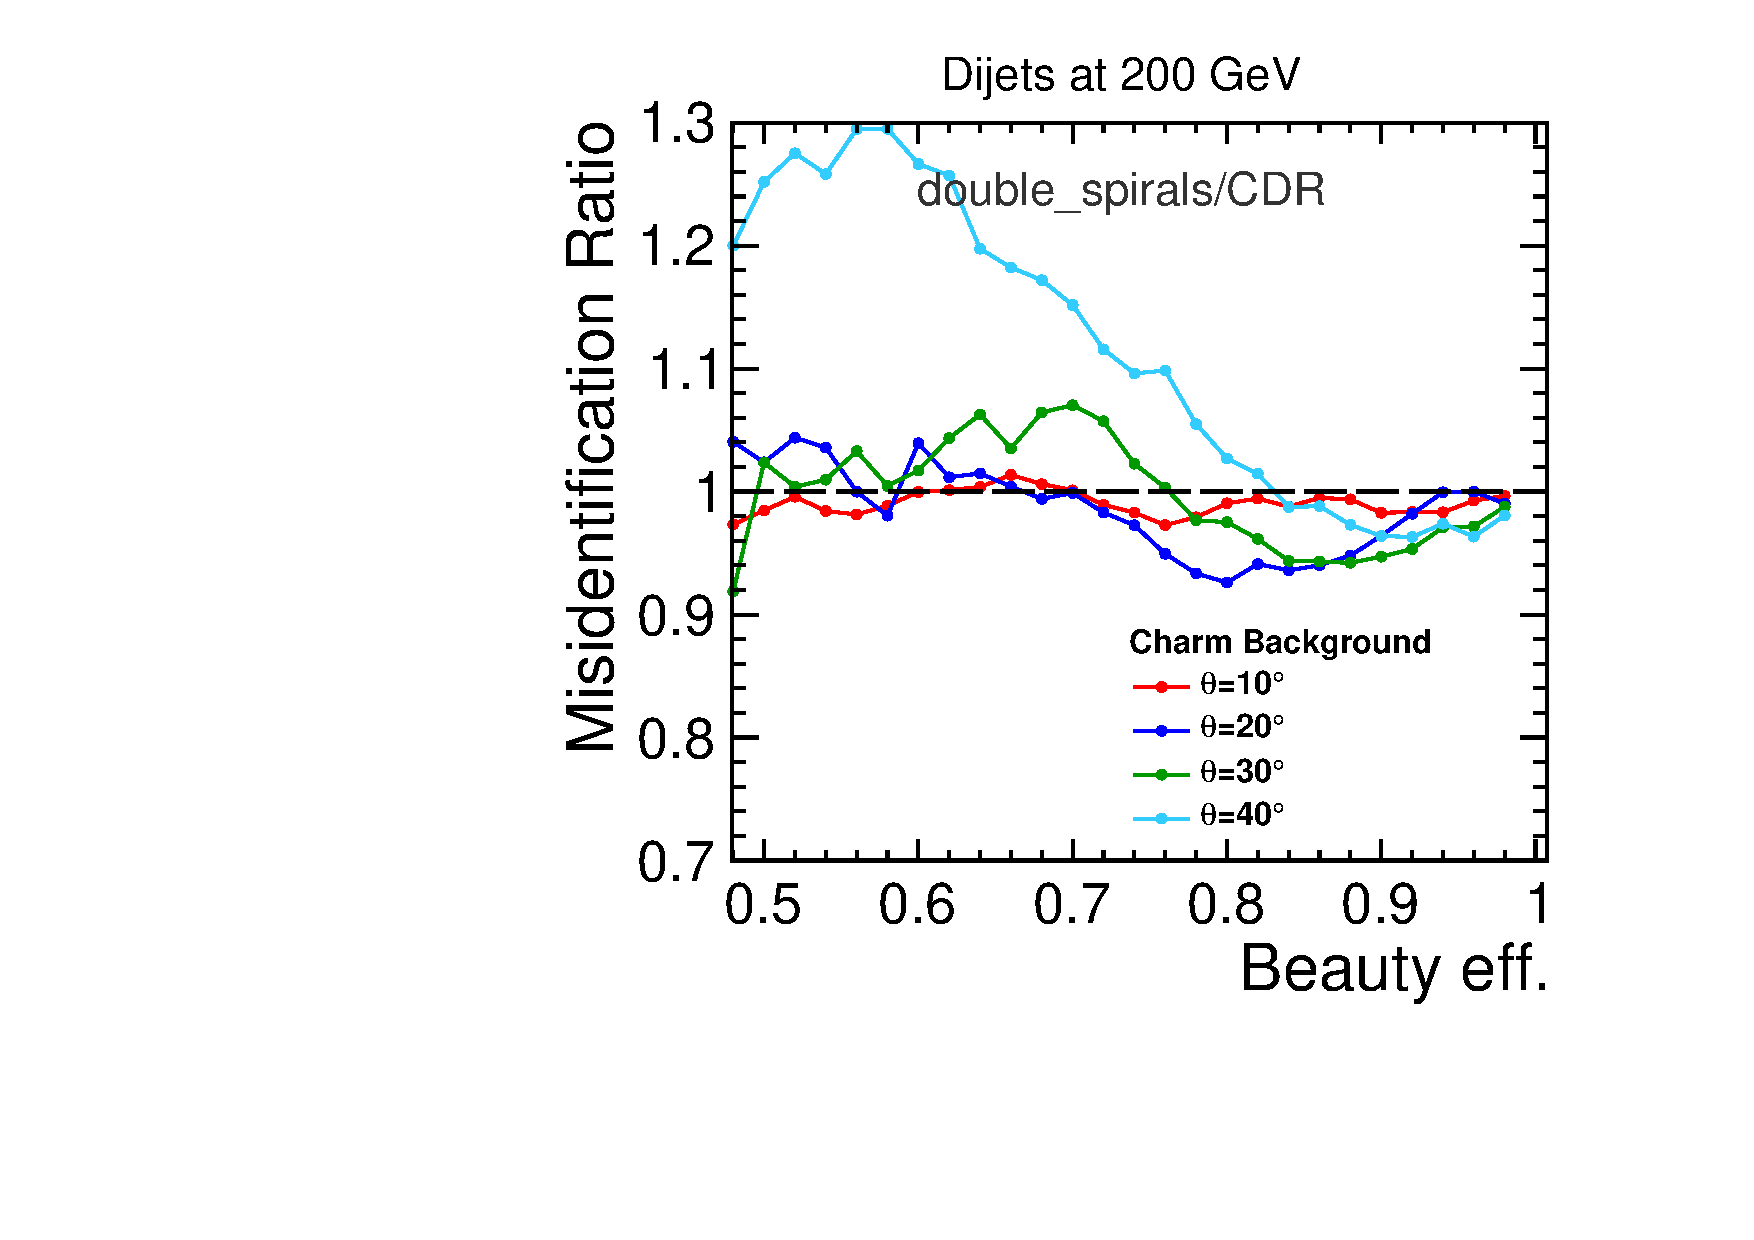
\includegraphics[width=\textwidth]{Figures/ImpactOfGeometries/200GeV_Ratio_allAngles_doubleSpirals_CDR_B_C.pdf}};
      \draw[white, fill=white] (1.8, 6.3) rectangle (5.7, 7);
    \end{tikzpicture}
    \caption{}
    \label{}
  \end{subfigure}%
  ~ 
  \begin{subfigure}[b]{0.5\textwidth}
    \centering
    \begin{tikzpicture}
      \node[anchor=south west,inner sep=0] (image) at (0,0){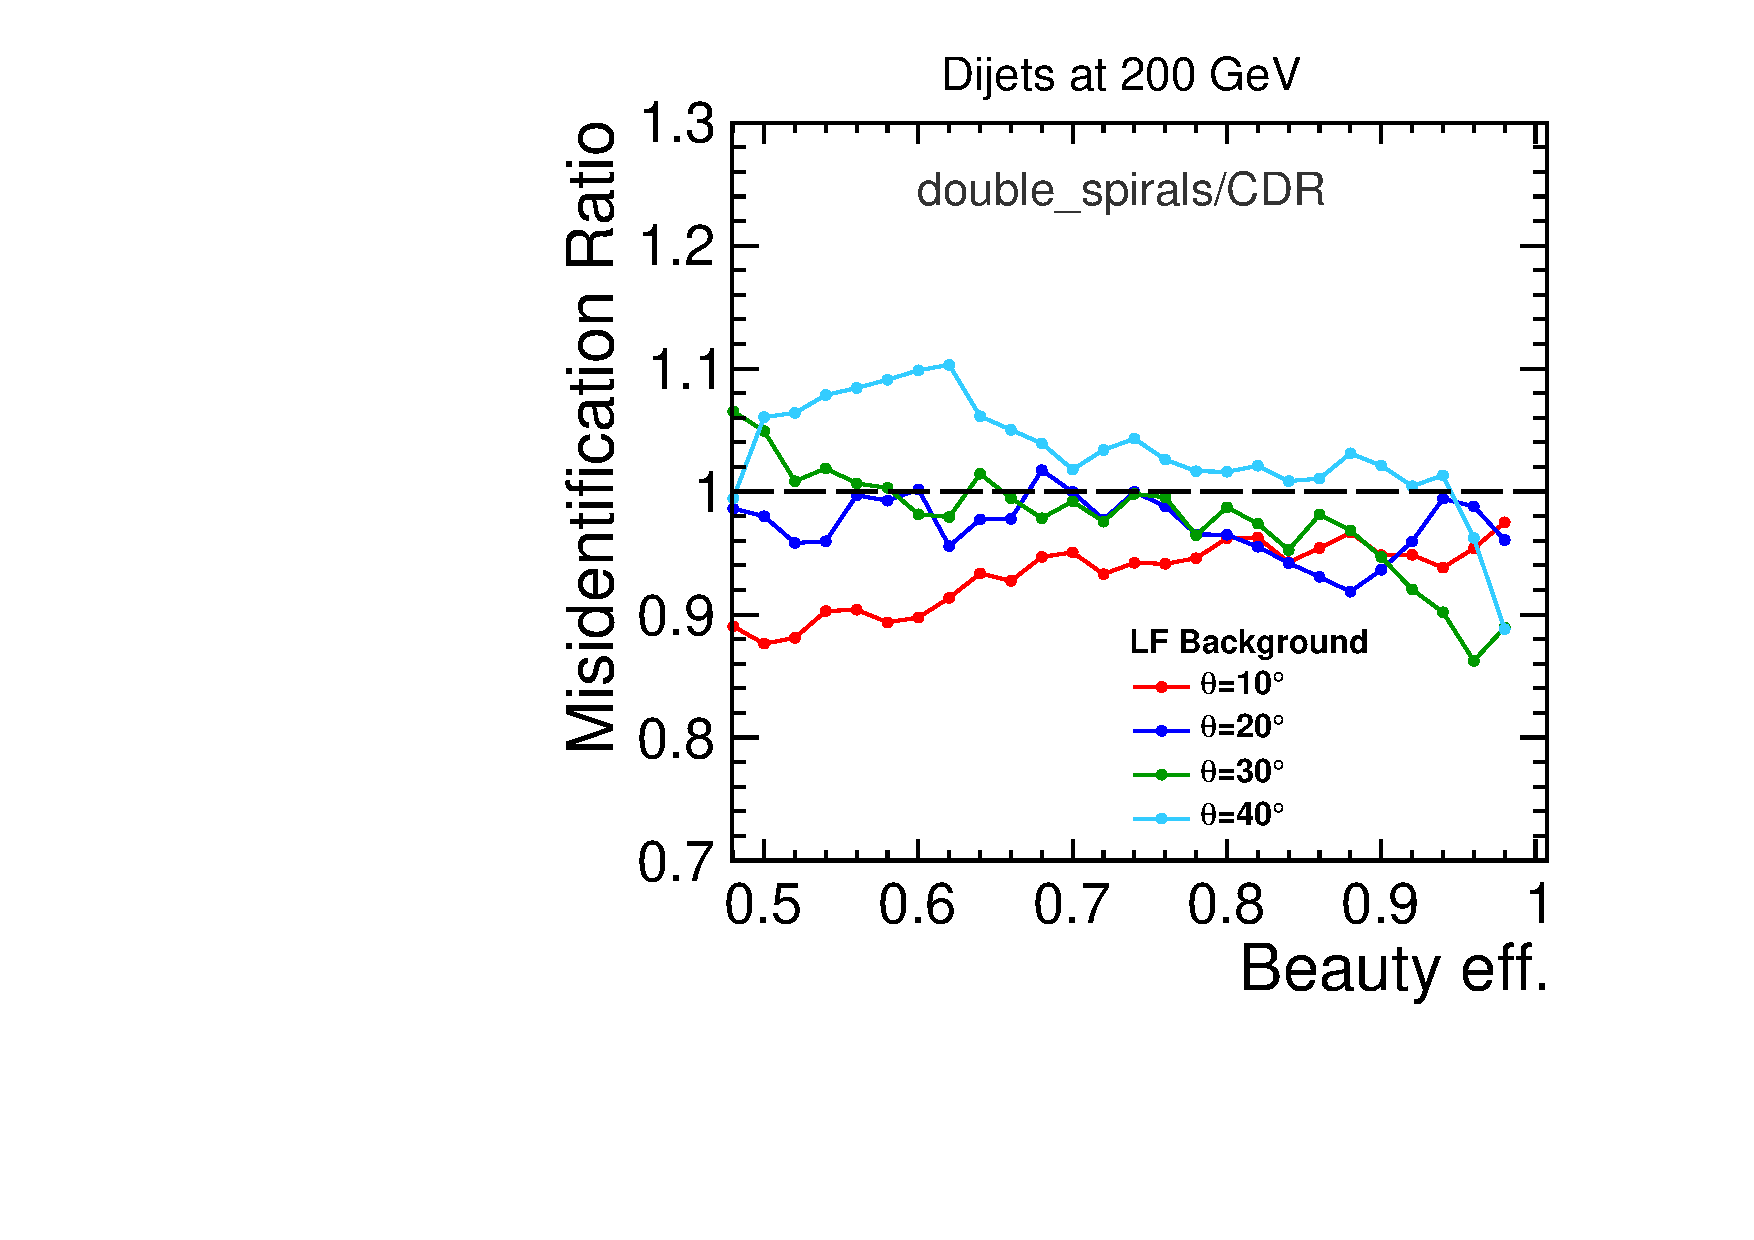
\includegraphics[width=\textwidth]{Figures/ImpactOfGeometries/200GeV_Ratio_allAngles_doubleSpirals_CDR_B_LF.pdf}};
      \draw[white, fill=white] (1.8, 6.3) rectangle (5.7, 7);
    \end{tikzpicture}
    \caption{}
    \label{}
  \end{subfigure}
  \caption{The ratios between the misidentification
    probabilities for the \textit{double\_spirals} and the CDR geometries
    as function of the b-tag efficiency considering the charm
    (a) and the light flavour (b) backgrounds based on jets in dijet events at $\sqrt{s}=200$~GeV.}\label{fig:double_disks_beauty}
\end{figure}

\begin{figure}[H]
  \begin{subfigure}[b]{0.5\textwidth}
    \centering
    \begin{tikzpicture}
      \node[anchor=south west,inner sep=0] (image) at (0,0){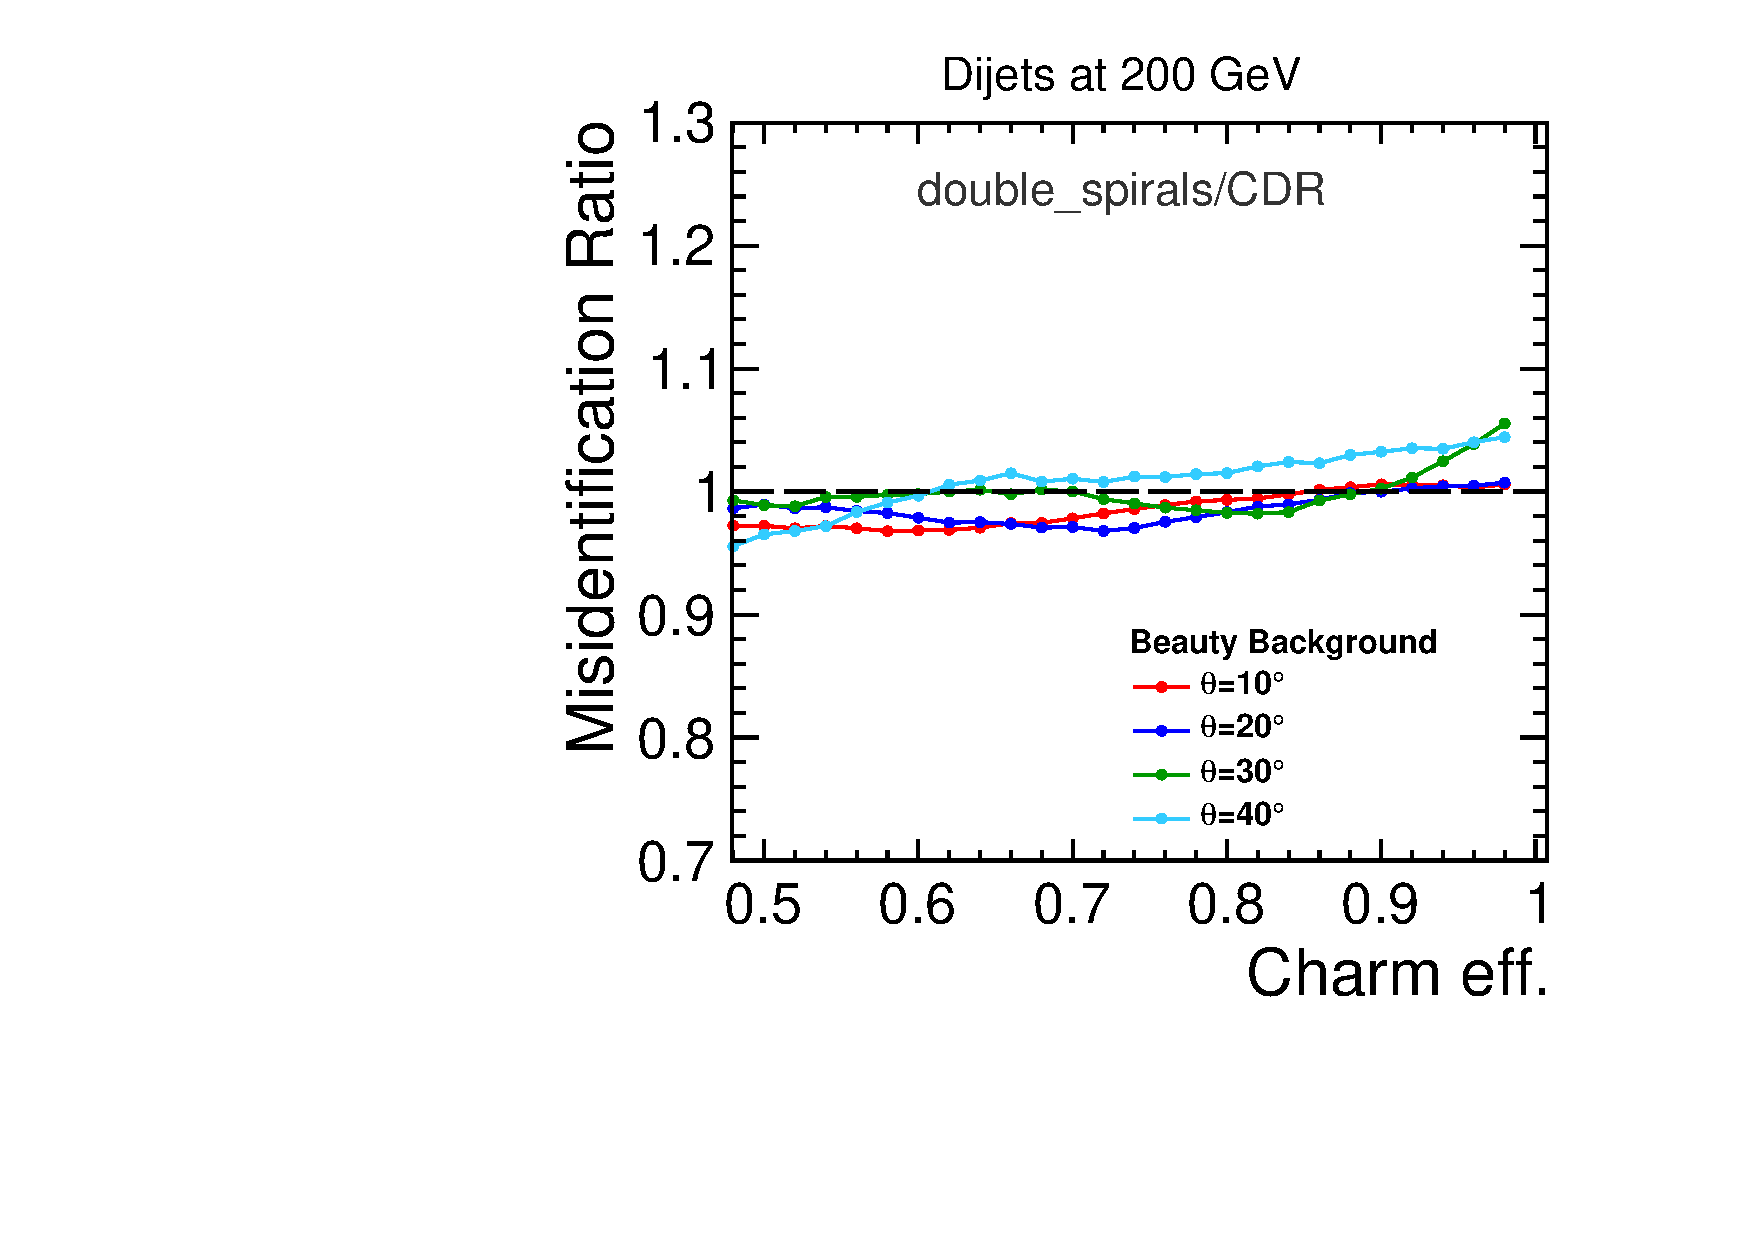
\includegraphics[width=\textwidth]{Figures/ImpactOfGeometries/200GeV_Ratio_allAngles_doubleSpirals_CDR_C_B.pdf}};
      \draw[white, fill=white] (1.8, 6.3) rectangle (5.7, 7);
    \end{tikzpicture}
    \caption{}
    \label{}
  \end{subfigure}%
  ~ 
  \begin{subfigure}[b]{0.5\textwidth}
    \centering
    \begin{tikzpicture}
      \node[anchor=south west,inner sep=0] (image) at (0,0){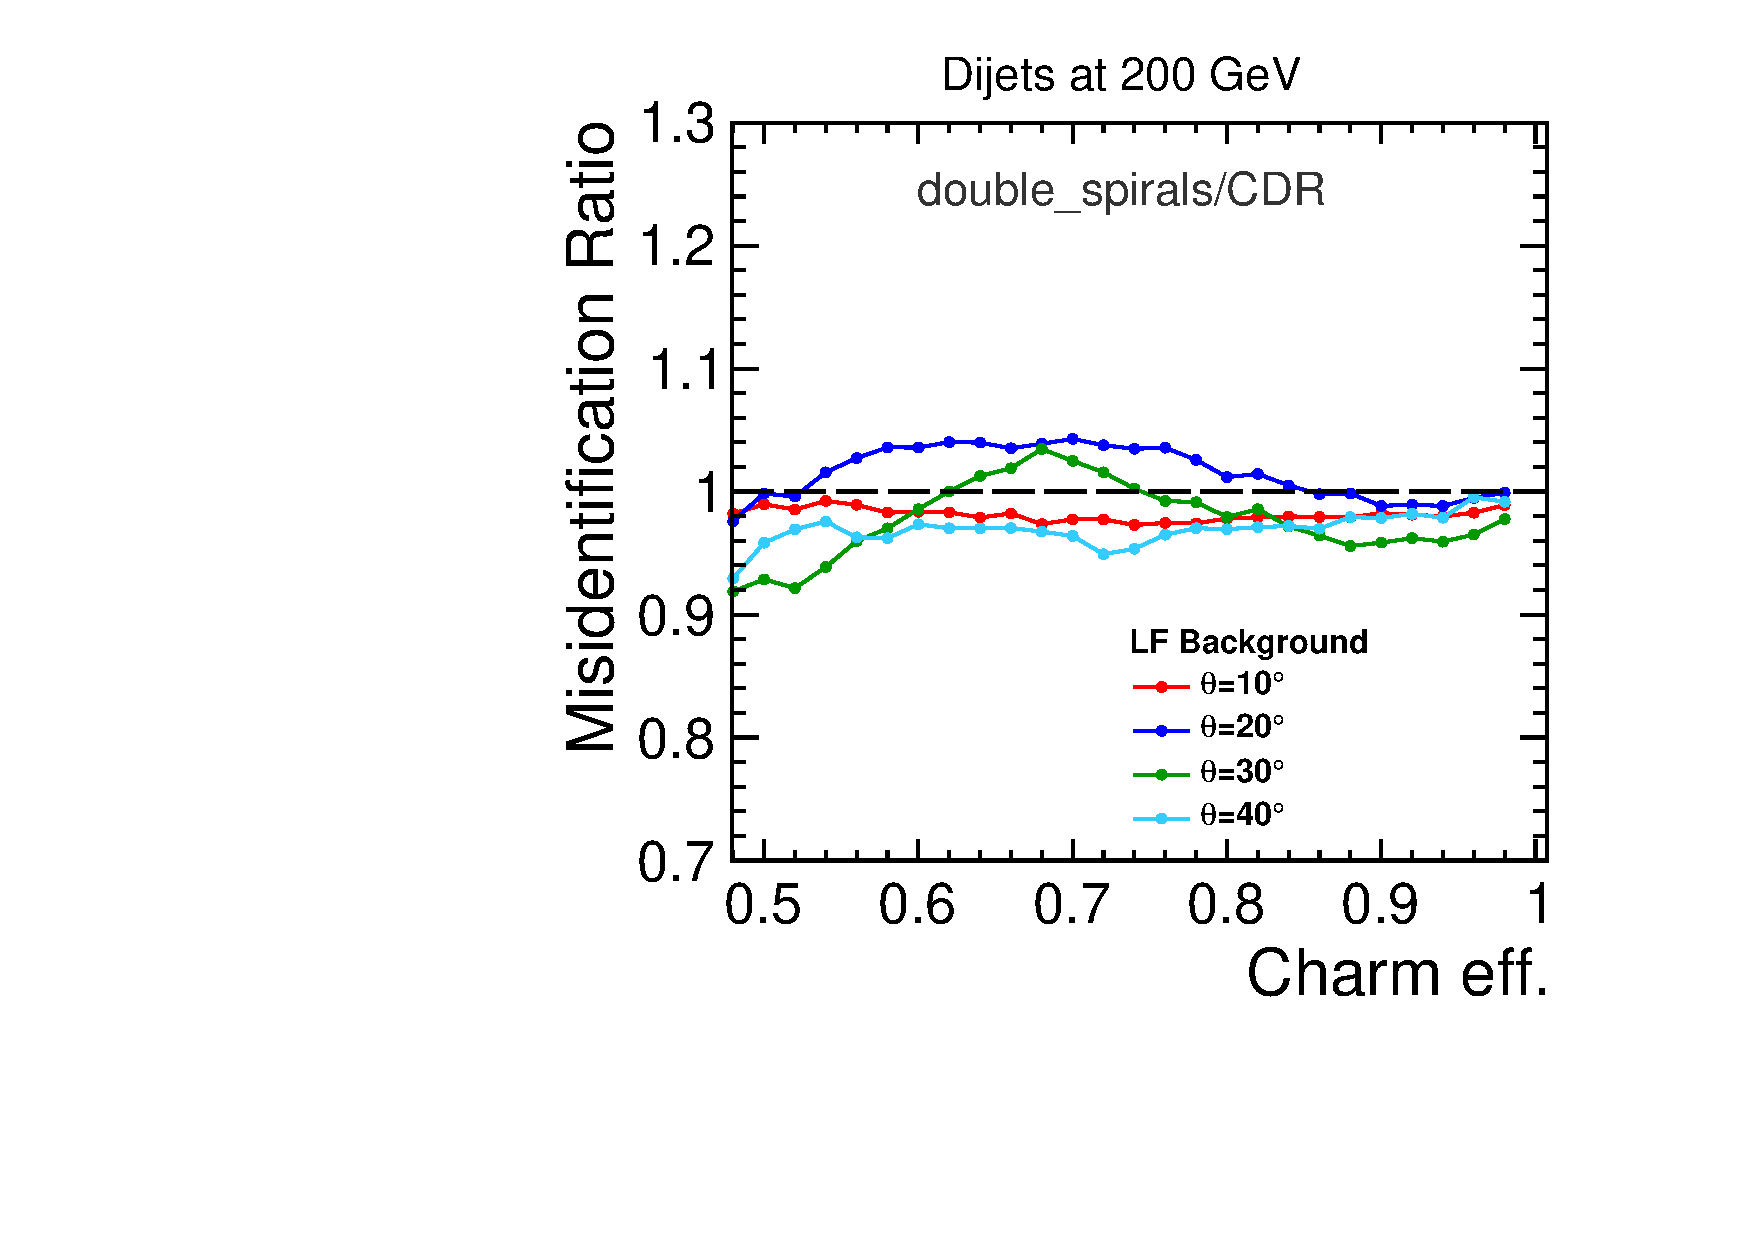
\includegraphics[width=\textwidth]{Figures/ImpactOfGeometries/200GeV_Ratio_allAngles_doubleSpirals_CDR_C_LF.pdf}};
      \draw[white, fill=white] (1.8, 6.3) rectangle (5.7, 7);
    \end{tikzpicture}
    \caption{}
    \label{}
  \end{subfigure}
  \caption{The ratios between the misidentification
    probabilities for the \textit{double\_spirals} and the CDR geometries
    as function of the c-tag efficiency considering the beauty
    (a) and the light flavour (b) backgrounds based on jets in dijet events at $\sqrt{s}=200$~GeV.}\label{fig:double_disks_charm}
\end{figure}



\subsection{Impact of the material budget}\label{sec:impactOfMaterialBudget}

The {\it double\_spirals\_v2} geometry is a more realistic version of
the {\it double\_spirals} geometry, taking into account the material
used for the mechanical support of the sensors and also the material
used for the cables. The material budget per double layer is 0.4\%~X$_{0}$.
The flavour-tagging performance of this geometry is given in Figure~\ref{fig:heavy_200} and compared to the \textit{double\_spirals} layout. Dijet events
with a mixture of polar angles between $10^{\circ}$ and $90^{\circ}$ are used for the flavour tagging.\\
By increasing the material in the vertex detector, the fake rate increases by approximately 5-35\% depending on the
required signal efficiency and background type.


\begin{figure}[H]
  \begin{subfigure}[b]{0.5\textwidth}
    \centering
    \begin{tikzpicture}
      \node[anchor=south west,inner sep=0] (image) at (0,0){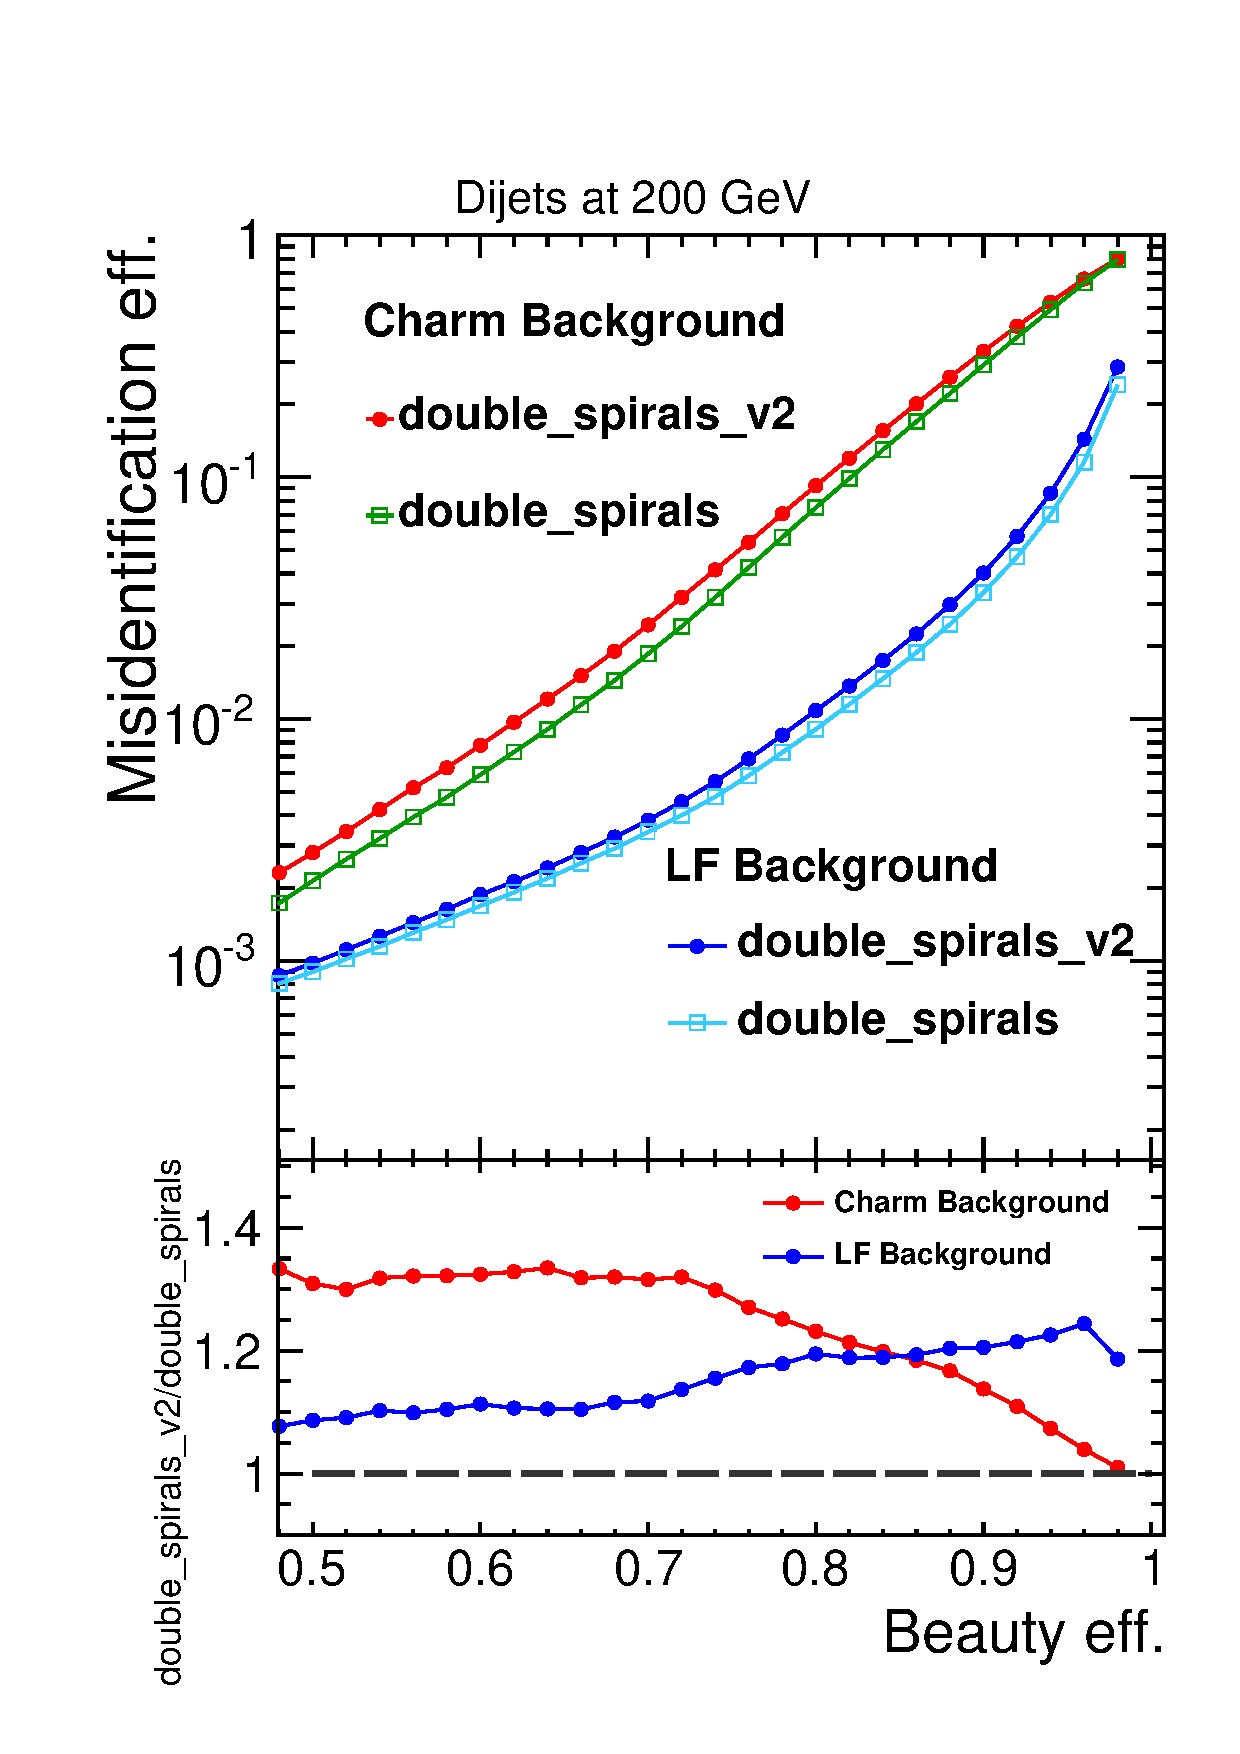
\includegraphics[width=\textwidth]{Figures/ImpactOfGeometries/heavy_general_200_Beauty.pdf}};
      \draw[white, fill=white] (1.8, 9.95) rectangle (5.5, 10.6);
    \end{tikzpicture}
    \caption{}
    \label{}
  \end{subfigure}%
  ~ 
  \begin{subfigure}[b]{0.5\textwidth}
    \centering
    \begin{tikzpicture}
      \node[anchor=south west,inner sep=0] (image) at (0,0){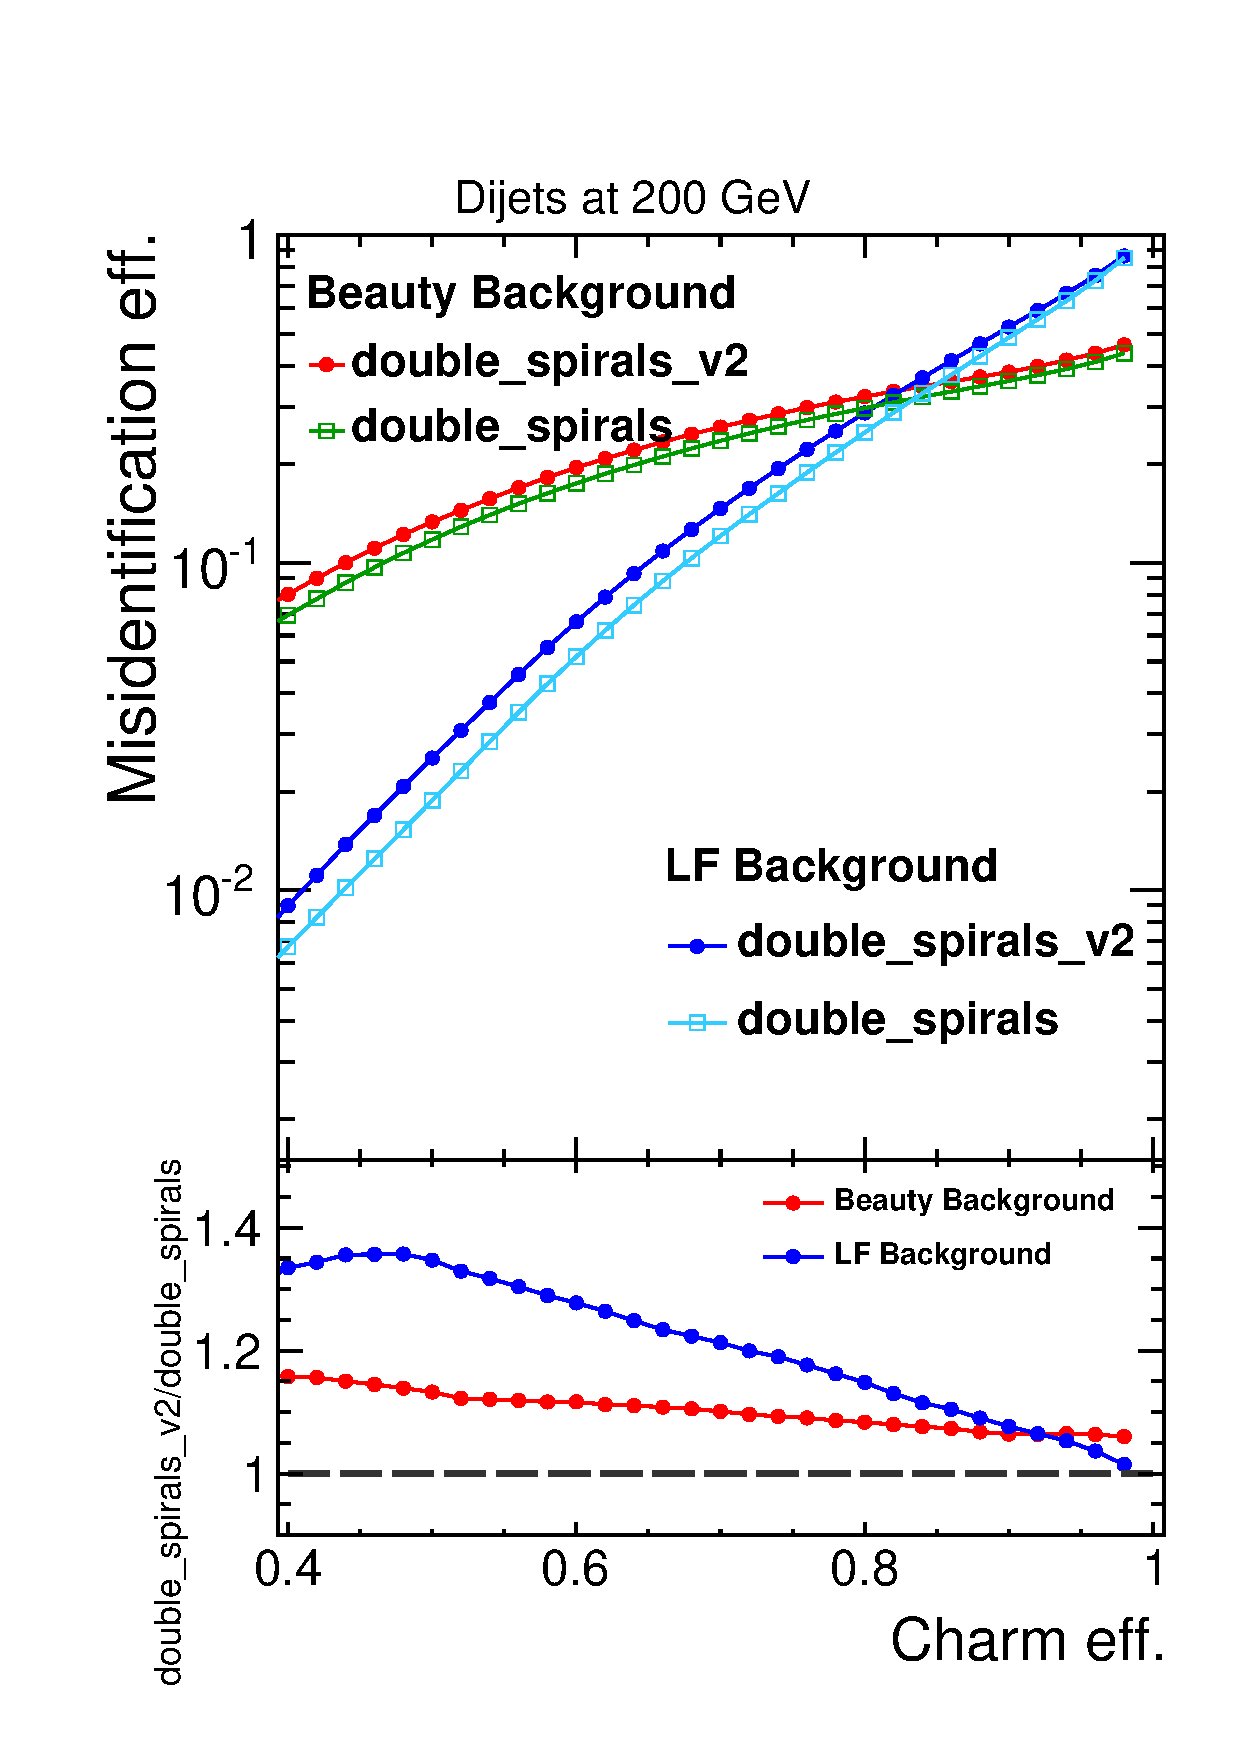
\includegraphics[width=\textwidth]{Figures/ImpactOfGeometries/heavy_general_200_Charm.pdf}};
      \draw[white, fill=white] (1.8, 9.95) rectangle (5.5, 10.6);
    \end{tikzpicture}
    \caption{}
    \label{}
  \end{subfigure}
  \caption{Global comparison between the \textit{double\_spirals\_v2} and
    the \textit{double\_spirals} geometries based on beauty tagging (a)
    and charm tagging (b) for jets in dijet events at $\sqrt{s}=$200~GeV with a
    mixture of polar angles between $10^{\circ}$ and
    $90^{\circ}$. On the y-axis, the misidentification probability
    and the ratio between the misidentification probabilities for
    the two geometries are given.}\label{fig:heavy_200}
\end{figure}

%----------------------------------------------------------------------

